 % -*- Mode:TeX -*-

%% IMPORTANT: The official thesis specifications are available at:
%%            http://libraries.mit.edu/archives/thesis-specs/
%%
%%            Please verify your thesis' formatting and copyright
%%            assignment before submission.  If you notice any
%%            discrepancies between these templates and the 
%%            MIT Libraries' specs, please let us know
%%            by e-mailing thesis@mit.edu

%% The documentclass options along with the pagestyle can be used to generate
%% a technical report, a draft copy, or a regular thesis.  You may need to
%% re-specify the pagestyle after you \include  cover.tex.  For more
%% information, see the first few lines of mitthesis.cls. 

%\documentclass[12pt,vi,twoside]{mitthesis}
%%
%%  If you want your thesis copyright to you instead of MIT, use the
%%  ``vi'' option, as above.
%%
%\documentclass[12pt,twoside,leftblank]{mitthesis}
%%
%% If you want blank pages before new chapters to be labelled ``This
%% Page Intentionally Left Blank'', use the ``leftblank'' option, as
%% above. 

\documentclass[12pt,twoside]{mitthesis}
\usepackage{lgrind}
\usepackage{graphicx}
\usepackage{url}
%% These have been added at the request of the MIT Libraries, because
%% some PDF conversions mess up the ligatures.  -LB, 1/22/2014
\usepackage{cmap}
\usepackage[T1]{fontenc}
\usepackage{subcaption}
\usepackage{tikz,pgfplots}
\pgfplotsset{compat=1.14}
\usepackage{wasysym}

\pagestyle{plain}

%% This bit allows you to either specify only the files which you wish to
%% process, or `all' to process all files which you \include.
%% Krishna Sethuraman (1990).

%%\typein [\files]{\include{all}}
%%\def\all{all}
%%\ifx\files\all \typeout{Including all files.} \else \typeout{Including only \files.} \includeonly{\files} \fi

\newlength\figureheight 
\newlength\figurewidth 

\begin{document}

% -*-latex-*-
% 
% For questions, comments, concerns or complaints:
% thesis@mit.edu
% 
%
% $Log: cover.tex,v $
% Revision 1.8  2008/05/13 15:02:15  jdreed
% Degree month is June, not May.  Added note about prevdegrees.
% Arthur Smith's title updated
%
% Revision 1.7  2001/02/08 18:53:16  boojum
% changed some \newpages to \cleardoublepages
%
% Revision 1.6  1999/10/21 14:49:31  boojum
% changed comment referring to documentstyle
%
% Revision 1.5  1999/10/21 14:39:04  boojum
% *** empty log message ***
%
% Revision 1.4  1997/04/18  17:54:10  othomas
% added page numbers on abstract and cover, and made 1 abstract
% page the default rather than 2.  (anne hunter tells me this
% is the new institute standard.)
%
% Revision 1.4  1997/04/18  17:54:10  othomas
% added page numbers on abstract and cover, and made 1 abstract
% page the default rather than 2.  (anne hunter tells me this
% is the new institute standard.)
%
% Revision 1.3  93/05/17  17:06:29  starflt
% Added acknowledgements section (suggested by tompalka)
% 
% Revision 1.2  92/04/22  13:13:13  epeisach
% Fixes for 1991 course 6 requirements
% Phrase "and to grant others the right to do so" has been added to 
% permission clause
% Second copy of abstract is not counted as separate pages so numbering works
% out
% 
% Revision 1.1  92/04/22  13:08:20  epeisach

% NOTE:
% These templates make an effort to conform to the MIT Thesis specifications,
% however the specifications can change.  We recommend that you verify the
% layout of your title page with your thesis advisor and/or the MIT 
% Libraries before printing your final copy.
\title{Autonomous Grasping of Dynamic Objects}

\author{Patrick Lynch}
% If you wish to list your previous degrees on the cover page, use the 
% previous degrees command:
%       \prevdegrees{A.A., Harvard University (1985)}
% You can use the \\ command to list multiple previous degrees
%       \prevdegrees{B.S., University of California (1978) \\
%                    S.M., Massachusetts Institute of Technology (1981)}
\department{Department of Mechanical and Manufacturing Engineering}

% If the thesis is for two degrees simultaneously, list them both
% separated by \and like this:
% \degree{Doctor of Philosophy \and Master of Science}
\degree{Bachelor of Science in Computer Science and Engineering}

% As of the 2007-08 academic year, valid degree months are September, 
% February, or June.  The default is June.
\degreemonth{June}
\degreeyear{1990}
\thesisdate{May 18, 1990}

%% By default, the thesis will be copyrighted to MIT.  If you need to copyright
%% the thesis to yourself, just specify the `vi' documentclass option.  If for
%% some reason you want to exactly specify the copyright notice text, you can
%% use the \copyrightnoticetext command.  
%\copyrightnoticetext{\copyright IBM, 1990.  Do not open till Xmas.}

% If there is more than one supervisor, use the \supervisor command
% once for each.
\supervisor{Dr Conor McGinn}{Assistant Professor}

% This is the department committee chairman, not the thesis committee
% chairman.  You should replace this with your Department's Committee
% Chairman.
\chairman{Arthur C. Smith}{Chairman, Department Committee on Graduate Theses}

% Make the titlepage based on the above information.  If you need
% something special and can't use the standard form, you can specify
% the exact text of the titlepage yourself.  Put it in a titlepage
% environment and leave blank lines where you want vertical space.
% The spaces will be adjusted to fill the entire page.  The dotted
% lines for the signatures are made with the \signature command.
\maketitle

% The abstractpage environment sets up everything on the page except
% the text itself.  The title and other header material are put at the
% top of the page, and the supervisors are listed at the bottom.  A
% new page is begun both before and after.  Of course, an abstract may
% be more than one page itself.  If you need more control over the
% format of the page, you can use the abstract environment, which puts
% the word "Abstract" at the beginning and single spaces its text.

%% You can either \input (*not* \include) your abstract file, or you can put
%% the text of the abstract directly between the \begin{abstractpage} and
%% \end{abstractpage} commands.

% First copy: start a new page, and save the page number.
\cleardoublepage
% Uncomment the next line if you do NOT want a page number on your
% abstract and acknowledgments pages.
% \pagestyle{empty}
\setcounter{savepage}{\thepage}
\begin{abstractpage}
% $Log: abstract.tex,v $
% Revision 1.1  93/05/14  14:56:25  starflt
% Initial revision
% 
% Revision 1.1  90/05/04  10:41:01  lwvanels
% Initial revision
% 
%
%% The text of your abstract and nothing else (other than comments) goes here.
%% It will be single-spaced and the rest of the text that is supposed to go on
%% the abstract page will be generated by the abstractpage environment.  This
%% file should be \input (not \include 'd) from cover.tex.

% should be ~500 words

%% Background
Grasping moving objects is a challenging problem in the field of robotics. Traditional approaches are computationally expensive, over reliant on vision-based systems and often require an existing sensor infrastructure in the robot's environment. These make existing techniques unsuitable for implementation on mobile robotic platforms. The potential contribution of alternative strategies, in particular of other types of sensing, remains under-explored. 
%% Aims
The aim of this project is to investigate the role which sensing plays in the ability of a robot to grasp an object in motion. It is hypothesised that a sensor-heavy approach, where multiple sensing modalities are combined, can enable a robust grasping strategy, suited to implementation on a mobile robot.
%% Method
In order to test this hypothesis, the topic was broken into several research questions and addressed individually. In order to enable testing, a two-finger pincer gripper was designed and manufactured. To date, tests were performed on this pincer gripper with and without tactile sensing and their performances compared. A similar methodology will be employed in the future to investigate other sensing mechanisms, including vision and remote tactile.
%% Results and Conclusion
Tests have found that tactile feedback provided in real-time enabled the gripper to rapidly adapt to the moving object. This resulted in higher observed grasp robustness, in particular when the object's trajectory was offset from the center of the gripper. These findings indicate that tactile sensing can play an important role in informing the gripper motion when grasping moving objects and motivates further research on how the contribution of tactile sensing can be optimised and what other types of sensing might be utilised in creating a sensor-informed grasping motion for autonomous grasping of moving objects.

% conclusion, comment, contribution
% how have you added to field?




\end{abstractpage}

% Additional copy: start a new page, and reset the page number.  This way,
% the second copy of the abstract is not counted as separate pages.
% Uncomment the next 6 lines if you need two copies of the abstract
% page.
% \setcounter{page}{\thesavepage}
% \begin{abstractpage}
% % $Log: abstract.tex,v $
% Revision 1.1  93/05/14  14:56:25  starflt
% Initial revision
% 
% Revision 1.1  90/05/04  10:41:01  lwvanels
% Initial revision
% 
%
%% The text of your abstract and nothing else (other than comments) goes here.
%% It will be single-spaced and the rest of the text that is supposed to go on
%% the abstract page will be generated by the abstractpage environment.  This
%% file should be \input (not \include 'd) from cover.tex.

% should be ~500 words

%% Background
Grasping moving objects is a challenging problem in the field of robotics. Traditional approaches are computationally expensive, over reliant on vision-based systems and often require an existing sensor infrastructure in the robot's environment. These make existing techniques unsuitable for implementation on mobile robotic platforms. The potential contribution of alternative strategies, in particular of other types of sensing, remains under-explored. 
%% Aims
The aim of this project is to investigate the role which sensing plays in the ability of a robot to grasp an object in motion. It is hypothesised that a sensor-heavy approach, where multiple sensing modalities are combined, can enable a robust grasping strategy, suited to implementation on a mobile robot.
%% Method
In order to test this hypothesis, the topic was broken into several research questions and addressed individually. In order to enable testing, a two-finger pincer gripper was designed and manufactured. To date, tests were performed on this pincer gripper with and without tactile sensing and their performances compared. A similar methodology will be employed in the future to investigate other sensing mechanisms, including vision and remote tactile.
%% Results and Conclusion
Tests have found that tactile feedback provided in real-time enabled the gripper to rapidly adapt to the moving object. This resulted in higher observed grasp robustness, in particular when the object's trajectory was offset from the center of the gripper. These findings indicate that tactile sensing can play an important role in informing the gripper motion when grasping moving objects and motivates further research on how the contribution of tactile sensing can be optimised and what other types of sensing might be utilised in creating a sensor-informed grasping motion for autonomous grasping of moving objects.

% conclusion, comment, contribution
% how have you added to field?




% \end{abstractpage}

\cleardoublepage

\section*{Acknowledgments}

This is the acknowledgements section.  You should replace this with your
own acknowledgements.

%%%%%%%%%%%%%%%%%%%%%%%%%%%%%%%%%%%%%%%%%%%%%%%%%%%%%%%%%%%%%%%%%%%%%%
% -*-latex-*-

% Some departments (e.g. 5) require an additional signature page.  See
% signature.tex for more information and uncomment the following line if
% applicable.
% % -*- Mode:TeX -*-
%
% Some departments (e.g. Chemistry) require an additional cover page
% with signatures of the thesis committee.  Please check with your
% thesis advisor or other appropriate person to determine if such a 
% page is required for your thesis.  
%
% If you choose not to use the "titlepage" environment, a \newpage
% commands, and several \vspace{\fill} commands may be necessary to
% achieve the required spacing.  The \signature command is defined in
% the "mitthesis" class
%
% The following sample appears courtesy of Ben Kaduk <kaduk@mit.edu> and
% was used in his June 2012 doctoral thesis in Chemistry. 

\begin{titlepage}
\begin{large}
This doctoral thesis has been examined by a Committee of the Department
of Chemistry as follows:

\signature{Professor Jianshu Cao}{Chairman, Thesis Committee \\
   Professor of Chemistry}

\signature{Professor Troy Van Voorhis}{Thesis Supervisor \\
   Associate Professor of Chemistry}

\signature{Professor Robert W. Field}{Member, Thesis Committee \\
   Haslam and Dewey Professor of Chemistry}
\end{large}
\end{titlepage}


\pagestyle{plain}
% -*- Mode:TeX -*-
%% This file simply contains the commands that actually generate the table of
%% contents and lists of figures and tables.  You can omit any or all of
%% these files by simply taking out the appropriate command.  For more
%% information on these files, see appendix C.3.3 of the LaTeX manual. 
\tableofcontents
\newpage
\listoffigures
\newpage
\listoftables


% make sure to keep this 2-5 pages

%       Introduction
%
%   Opening Arguments
%       Justify Research
%
%   Introduces the Research
%   

\chapter{Introduction}

%% General paragraph introducing robotics as the topic and the trend towards applying them to new domains. Mentions service robots
Robots are becoming increasingly ubiquitous in a wide range of applications. Advances in robotics enable a growing range of features and increase the potential usefulness of the technology. Having been widely adapted in industrial applications for automation, there is increasing demand to apply robots elsewhere. Service robots are an example of this, it is increasingly common to see robots in entertainment, hospitality and health care applications. There are significant advantages associated with deploying robots in these domains. For example, robots can be used to increase the independence of older adults or people living with disabilities. However, with this ever expanding range of potential applications new challenges are presented. 

% What is the problem and why is it challenging, Structured vs unstructured environments

Robots, even relatively primitive platforms, perform well in highly-structured environments. Automation of manufacturing and assembly of products in industry using robots is largely a solved problem. In the case of manufacturing or assembly, the environment in which the robot is deployed is highly controlled and often designed specifically for the robot in question. A robot deployed for the automation of an assembly process does not need to be robust to lighting conditions, need to grasp something which is outside of it's manipulator's range, or consider that something, for example a human, might get in the path of its arm. This is not true of robots which are designed to work in less structured environments. A robot working in a hotel, building lobby or health care facility needs to be more adaptable. This adaptability requires a much higher level of complexity. There is a demand for a more flexible, adaptable robot.  

%% Introducing grasping moving objects

One area where this move to more unstructured and dynamic environments is particularly challenging is manipulation and grasping. Manipulation and grasping are essential functions of a general purpose robot. The ability to grasp and manipulate an object extends the robot's ability beyond sensing and navigating its environment to the ability to manipulate and interact with it's environment. In a controlled environment the problem is typically simplified by ensuring that a known object is in a known location and favourable orientation. When a robots needs to be able to effectively grasp in less structured environments this is not the case. Furthermore, the range of objects which a general purpose service robot would encounter and be expected to grasp is much larger. Finally, it is naive to assume that the objects which you will want to grasp will always be static and remain static throughout the interaction. This document outlines ongoing research which specifically examines the autonomous robotic grasping of dynamic objects.

\section{Background}

Robotic manipulation refers to a robots ability to interact with an object in its environment. It is the robotic equivalent a human using its arms and hands to interact with objects. This research is concerned  specifically with the end effector or gripper of the robot, i.e. mechanism at the end of a robotic manipulator. At a high level, robotic manipulation consists of 3 primary components, sensing, processing/planning and actuation. A wide variety of sensing manipulation and grasping strategies typically are just variations of these 3 core components. Sensing refers to how a robotic arm collects data about its environment, including the target object. Processing or planning refers to how the system analyses that sensory input and decides on an appropriate response. There are a variety of approaches to planning, ranging from reactive strategies to planning strategies, these will be discussed more later. Finally, Actuation is the physical movement of the robotic system in an attempt to achieve the goal.

Grasping is considered by some to be a solved problem \cite{APCObservations}, others have said that it's technology readiness level (TRL) should be considered between a 3 and a 4 \cite{KukayouBot} (TRL is a scale between 1 and 9). This disagreement about the current state of the art in grasping stems from the context in which the grasping is implemented. Grasping in structured environments is largely considered a solved problem. The type of grasping which has be deemed between a 3 and 4 technology readiness level refers to grasping on a professional service robot or a robot in a flexible cognitive manufacturing scenario. In other words robots operating in less structured environments. This is a distinction which is very important in grasping and in this project.


\subsection{Challanges}

Despite the maturity of manipulation and grasping research, there are persistent challenges which researchers have been striving to overcome for decades and are still not satisfactorily solved. The most commonly encountered include:
\begin{itemize}
    \item Unstructured Environments \cite{Delft, Zhao}
    
    Unstructured environments is a problem common to robotics and is mentioned above. It is particularly relevant in grasping where traditionally a complex problem has been simplified though the use of assumptions. In unstructured environments it is not effective to assume there are no obstacles between the robot and target object, or that the object is static. Creating a robotic gripper which is effective in unstructured environments is a very difficult problem.
    \item Occlusion \cite{Delft, Detectionandmapping, Zhao}
    
    Traditionally grasping problems have relied heavily on vision sensing. Vision sensing enables the passive collection of large amounts of accurate data about the environment. Robotics relies heavily on vision for grasping, mostly for the same reasons which humans rely heavily on their vision. Unfortunately, vision sensing is inherently vulnerable to occlusion problems, particularly in grasping applications where the gripper itself tends to occluded any on-board vision sensors. In humans, this shortcoming is overcome by using other senses.
    \item Lighting Conditions \cite{Delft, Detectionandmapping}
    
    Sensitivity to different lighting conditions is a common problem in computer vision. A reliance on vision sensors make it a problem in robotics also. Conditions which are too bright or too dark can often cause problem during manipulation.
    \item Computation
    
    The computational demands of a grasping task range from very simple sensing and motor control to computationally demanding computer vision and path planning algorithms. This is of particular concern on mobile platforms where computation may be a limited resource.
    \item Latency
    
    Latency can pose a significant problem when conducting time critical tasks, such as grasping moving objects. Latency can be introduced at both a software and hardware level. In software there is a non trivial amount of time needed to analysis sensor data and compute an appropriate action. Similarly, when an appropriate action is determined a non-trivial amount of time is required for the robotic system to carry out that action, for example to reach a target position.
    
    
\end{itemize}


% research questions
\section{Research Questions}
This research project aim to address the following research questions.
\begin{itemize}
\item How can the grasping motion of the robotic gripper be optimised to grasp moving objects. 
\item Can tactile sensing enable a reactive grasping strategy and offer an increase in grasping success rate 
\item How can image sensors contribute to informing the grasping motion of a robotic gripper when grasping a moving object
\item Can a neural network be used to couple sensor stimulus to grasping actuators to achieve a more robust grasp
\item Can reinforcement learning be used to train such a neural network
\item Can alternative sensing modalities be used to optimise gripper motion when grasping a moving object
\end{itemize}

% aims and hypothesis
\section{Aims and Objectives}
The primary aims of this research include:

\begin{itemize}
    
\item Present a grasping strategy for the control of robot fingers based on feedback from a) embedded tactile sensors b) remote tactile sensors
\item Train a neural network to take sensor data as an input and control the grasping motion as an output
\item Investigate the role of image sensor placement while grasping a moving object.
\item Propose a visuotactile grasping system capable of robustly grasping moving objects
\end{itemize}

% document outline
\section{Document Outline}
Chapter 2 will present a comprehensive outline of the existing research and associated literature relevant to this challenge and give a sense of the current state of the art. Chapter 3 will present a gripper which was designed and manufactured during this project for the purposes of addressing the aforementioned research questions. Chapter 4 will present a tactile sensor, inspired by literature and created during this project to address research questions related to tactile sensing. Chapter 5 describes controlled experiments which were conducted and their corresponding results. These explore the ability of tactile sensing to enable a reactive gripper motion for grasping moving objects. Chapter 6, supported by several important appendices, will outline the plan for the rest of this research project. Showing granularity such as week by week timeline predictions, outline of experiments, methods and equipment required and plans for publications.




\chapter{Literature Review}\label{LitReview}

This research will focus on general purpose robots, operating in unstructured environments. More specifically it will focus on the grasping of dynamic objects. This section will outline existing research in grasping and grasping of dynamic objects. It will also explore related areas such as tactile servoing, robotic competitions, gripper design and more. It is through exploration of this prior research that the subject and direction of this project was informed.

%% Below stuff seems a little out place

Grasping is considered by some to be a solved problem \cite{APCObservations}, others have said that it's technology readiness level should be considered between a 3 and a 4 \cite{KukayouBot}. This disagreement about the current state of the art in grasping stems from the context in which the grasping is implemented. Grasping in structured environments is largely considered a solved problem. The type of grasping which has be deemed between a 3 and 4 technology readiness level refers to grasping on a professional service robot or a robot in a flexible cognitive manufacturing scenario. In other words robots operating in less structured environments. This is a distinction which is very important in grasping and in this project.

Grasping in structured environments is tackled by simplifying the grasping problem. Assumptions can be made about the shape, location, weight, size, and other characteristics of the target object and environment. This leads to a highly effective and robust grasping operation in that context but a solution which is ultimately very sensitivity to changes and unsuitable for implementation on a general purpose robot, operating in an unstructured environment.

%%%%%%%%%%%%%%

\section{Existing Grippers}

There is a large and diverse range of existing robotic grippers, visible both in research and in industry. These gripper vary widely from simplistic to complex and from general purpose to having a very specific, niche applications. It would be difficult to complete a comprehensive review of all available grippers, however this section aims to introduce a subset, representative of the current state of the art. Inspired and expanding on the categories given by \cite{APCinhandproxandcontact}, grippers are discussed under the following headings and real world examples of each are given.


\begin{itemize}
    \item Pincer Grippers \ref{fig:YouBot}, \ref{label:Robotiq85}, \ref{label:Hand-E}
    
    Pincer Grippers are one of the simplest types of gripper available. Despite their simplicity they are capable of a wide range of tasks. The result of low complexity and large application range is that they are one of the most used gripper morphologies. Pincer grippers use 2 opposing fingers to apply a clamping force onto the object. They require low control complexity but are inheriently limited and can encounter problems if the object is too large, heavy or irregularly shaped.
    
    \item Higher DOF Finger grippers \ref{lbel:Robotiq3Finger}
    
    These include robotic grippers with 3 or more fingers. Due to the larger number of fingers and therefore DOF the complexity, both mechanical and control, is higher. However, the number of grasp configurations which is possible also increases. These grippers have more potential as general purpose robotic gripper which could operate effectively in an unstructured environment, however due to their complexity they are more common in research than in industry. A comprehensive review of different types of grasp configurations is outside the scope of this document however has been explored in the literature previously \cite{GRASPTaxonomy}. The different finger configurations and associated grasps achievable with a 3-Fingered is explored by S. Tao, et. al \cite{Reconf3Finger}.
    
    
    \item Humanoid Grippers \ref{fig:Sandia}, \ref{fig:James}, \ref{fig:Allegro}, \ref{fig:DLR Hand II}
    
    Gripper morphologies which are similar to that of a human hand tend to operate very well in unstructured environments \cite{pneumaticAnthropomorphicHand,Mahmoud2010}. 
    This can be attributed to the fact that the human hand is an excellent general purpose tool, but also because many of the unstructured environments which we wish robots to operate in tend to have been designed for easy of use by humans. They are therefore generally well suited to robotic grippers of a similar size, shape, degrees of freedom, etc to a human hand. There other motivations to using a anthropomorphic gripper also. Their similarity aesthetically to a human hand makes them very desirable for prosthetics and they are desirable for applications where a gripper is tele-operated by a human since joint angles can be mapped directly from one to the other \cite{AnthroHandReview}.
    
    The downside of these types of grippers is their complexity. The large number of fingers/DOF makes control difficult. They also tend to be very mechanically complex due to the large number of actuators required to control the large number of DOF.
    
    \item Vacuum Grippers
    
    Suction cup grippers are a common robotic end effector. A vacuum gripper uses a vacuum to adhere to the surface of the target object. Their usefullness is fundementally limited by the range of objects which they can manipulate. It is not possible to create a gripper which relies solely on a vacuum mechanism which can generalise to an arbitrary shape. This was particularly evident at the amazon picking challenge where teams struggled to pick up a variety of objects such as books, mesh cups,toilet brush, pencils, sponge, clothing and marbles. when relying solely on a vacuum based gripper \cite{APCGripper, APCObservations}. Despite this they have proven very effective and therefore very common in grasping applications. During the 2018 Amazon Picking Challange 36\% of the teams used some for of suction \cite{APCObservations}. They have proven popular in more structured environments where the object is consistent and an appropriate grasping target for a vacuum gripper. Since they are simple and effective for a large range of objects they are often implemented in a hybrid configuration with a more traditional gripper \cite{Nakamoto2019} to overcome some of their shortcomings. A vacuum-pincer hybrid gripper was identified as a suitable candidate to grasp in the cluttered narrow spaces presented for grippers used for warehouse automation \cite{Hasegawa2017}. Team Delft, winners of the 2016 Amazon Picking Challange, used a hybrid pincer and vacuum gripper\cite{Delft}.
    
    \item Other \ref{fig:Coffee Bean Gripper}
    
    There are more examples of types of grippers, typically for niche applications. These are outside the scope of this research but for the sake of completeness will be mentioned here. The coffee bean gripper, seen in Fig. \ref{fig:Coffee Bean Gripper} uses a particle jamming mechanism to grasp objects. This technique is somewhat robust to different object geometries but struggles in some situations with grasp stability. The grasping procedure here is very simple, press the gripper on top of the object and activating the particle jamming by means of a vacuum pump to grasp the object. There is a reliance on the environment providing a reactant force when pressing on the object. Soft robotic grippers are also an active area of research \cite{RBOHand2}. These avoid using rigid components, substituting them instead for soft, passively compliant parts. These tend to be simpler to control, less expensive and inherently safe. However this typically comes at the cost of dexterity. The RBO hand 2 is shown in Fig \ref{fig:RBOHand2}.
    
\end{itemize}

\begin{figure}
    \centering
    \begin{subfigure}{.3\linewidth}
        \centering
 %   
\includegraphics[width=.4\textwidth]{Images/placeholder.png}       
    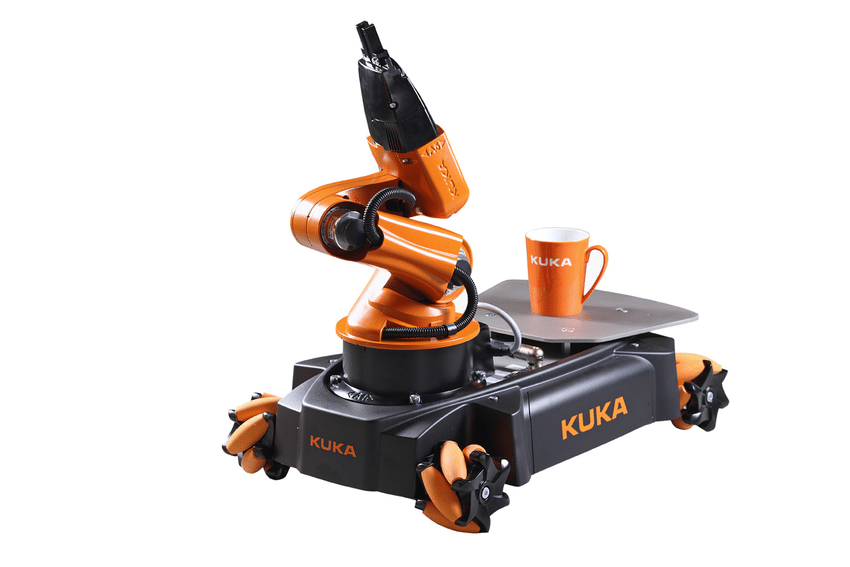
\includegraphics[width=0.7\textwidth]{Images/KukayouBot.png}
        \caption[youBot]{YouBot \cite{KukayouBot}}
        \label{fig:YouBot}
    \end{subfigure}
    \begin{subfigure}{.3\linewidth}
        \centering
        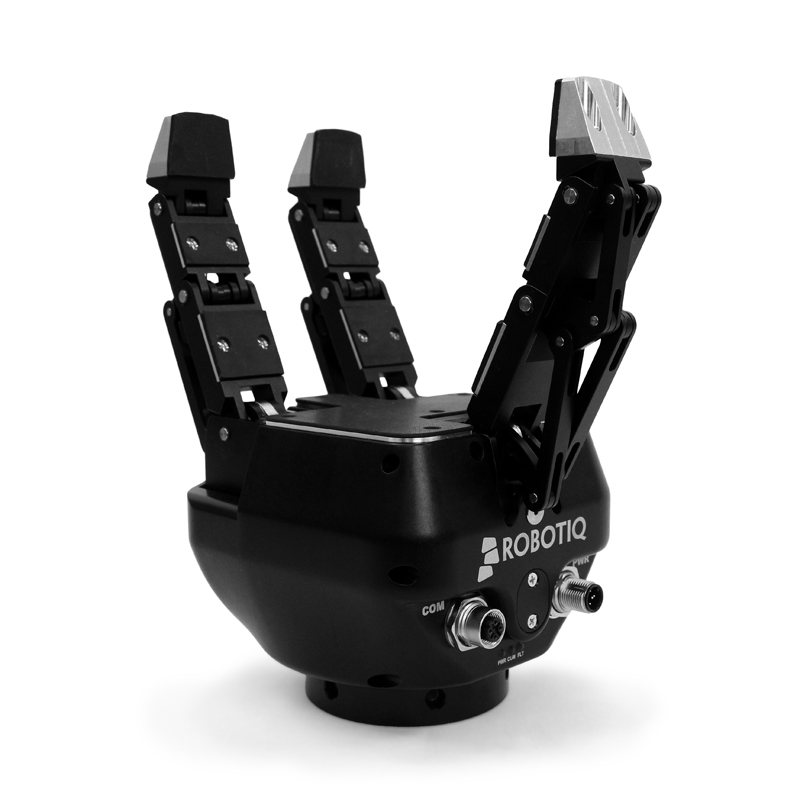
\includegraphics[width=0.7\textwidth]{Images/3-finger-robot-gripper-robotiq.jpg}
%    
\includegraphics[width=.4\textwidth]{Images/placeholder.png}
        \caption[3-Finger Adaptive Robot Gripper]{3-Finger Adaptive Robot Gripper \cite{RobotIQpic}}
        \label{lbel:Robotiq3Finger}
    \end{subfigure}
    \begin{subfigure}{.3\linewidth}
        \centering
%    
\includegraphics[width=.4\textwidth]{Images/placeholder.png}   
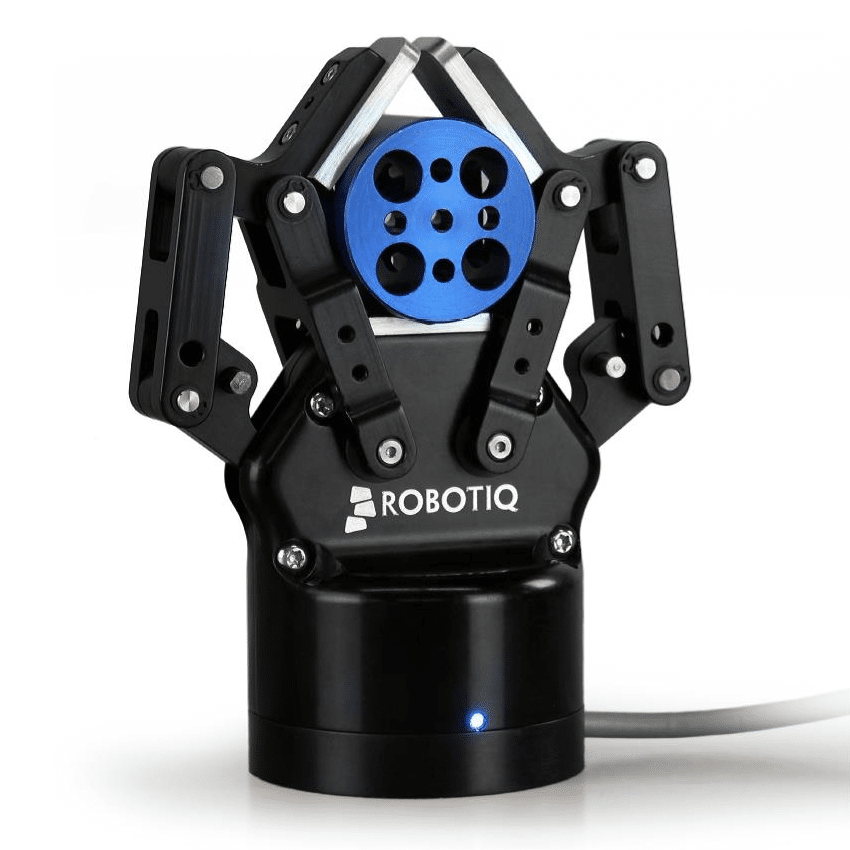
\includegraphics[width=0.7\textwidth]{Images/Robotiq-2-Finger-85-encompassing-grip.png}
        \caption[Robotiq 2F-85]{Robotiq 2F-85 \cite{RobotIQ2Fingerpic}}
        \label{label:Robotiq85}
    \end{subfigure}
    \begin{subfigure}{.3\linewidth}
        \centering
        \includegraphics[width=0.7\textwidth]{Images/Hand£.png}          
%    
\includegraphics[width=.4\textwidth]{Images/placeholder.png} 
        \caption[Robotiq Hand-E]{Robotiq Hand-E \cite{RobotIQHandEpic}}
        \label{label:Hand-E}
    \end{subfigure}
    \begin{subfigure}{.3\linewidth}
        \centering
        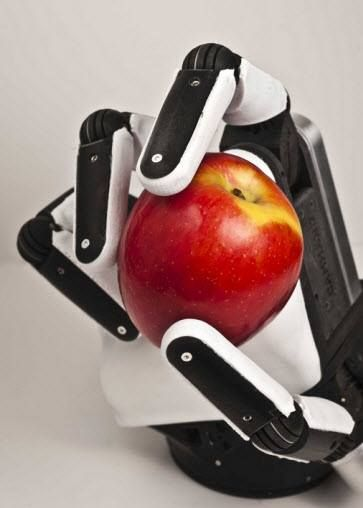
\includegraphics[width=0.7\textwidth]{Images/Sandia.jpg}       
  %  
\includegraphics[width=.4\textwidth]{Images/placeholder.png}
        \caption[Sandia Hand]{Sandia Hand \cite{SandiaHand}}
        \label{fig:Sandia}
    \end{subfigure}
    \begin{subfigure}{.3\linewidth}
        \centering
        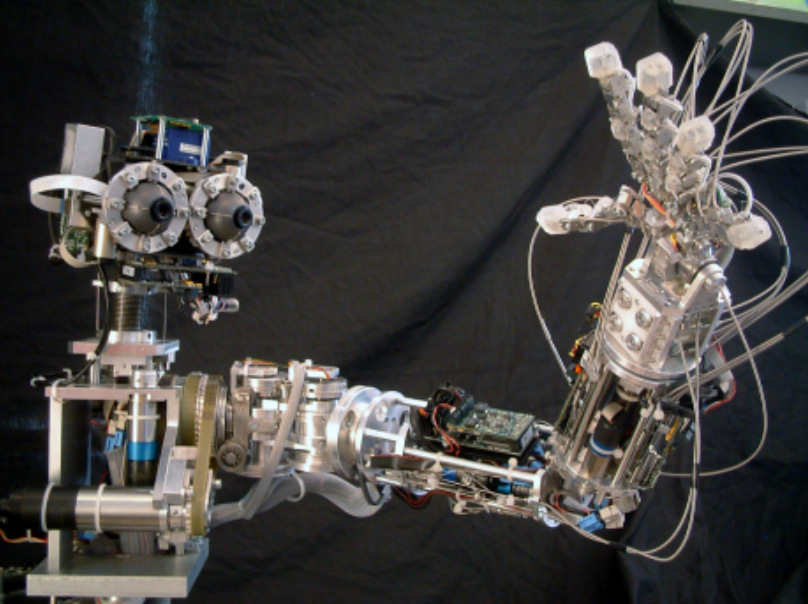
\includegraphics[width=0.7\textwidth]{Images/James.png}    
  %  
\includegraphics[width=.4\textwidth]{Images/placeholder.png}
        \caption[James]{James \cite{James}}
        \label{fig:James}
    \end{subfigure}
    \begin{subfigure}{.3\linewidth}
        \centering
        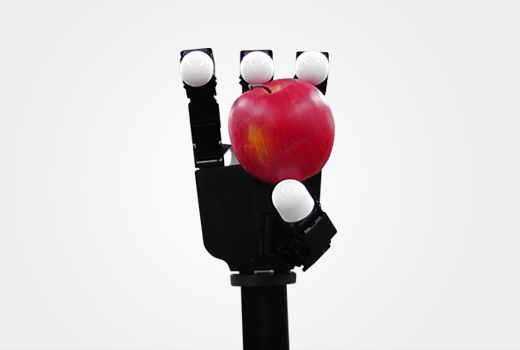
\includegraphics[width=0.7\textwidth]{Images/Allegro_Hand_flash_03.png}
 %   
\includegraphics[width=.4\textwidth]{Images/placeholder.png}
        \caption[Allegro Hand]{Allegro Hand \cite{AllegroHandpic}}
        \label{fig:Allegro}
    \end{subfigure}
    \begin{subfigure}{.3\linewidth}
        \centering
        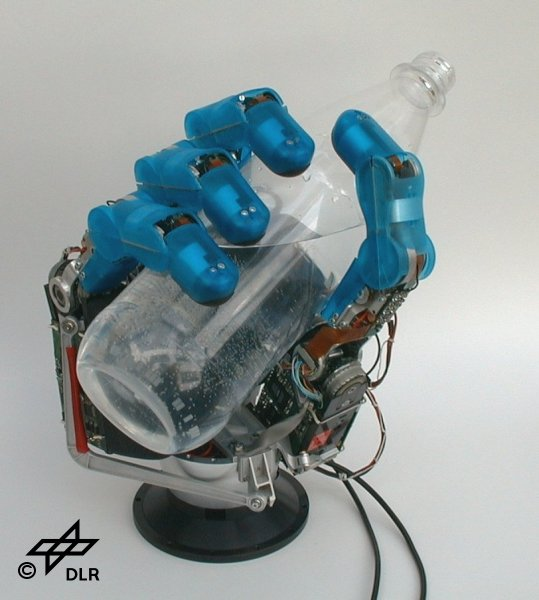
\includegraphics[width=0.7\textwidth]{Images/Hand-II-01.jpg}   
  %  
\includegraphics[width=.4\textwidth]{Images/placeholder.png}
        \caption[DLR Hand II]{DLR Hand II \cite{DLRHandIIpic}}
        \label{fig:DLR Hand II}
    \end{subfigure}
    \begin{subfigure}{.3\linewidth}
        \centering
      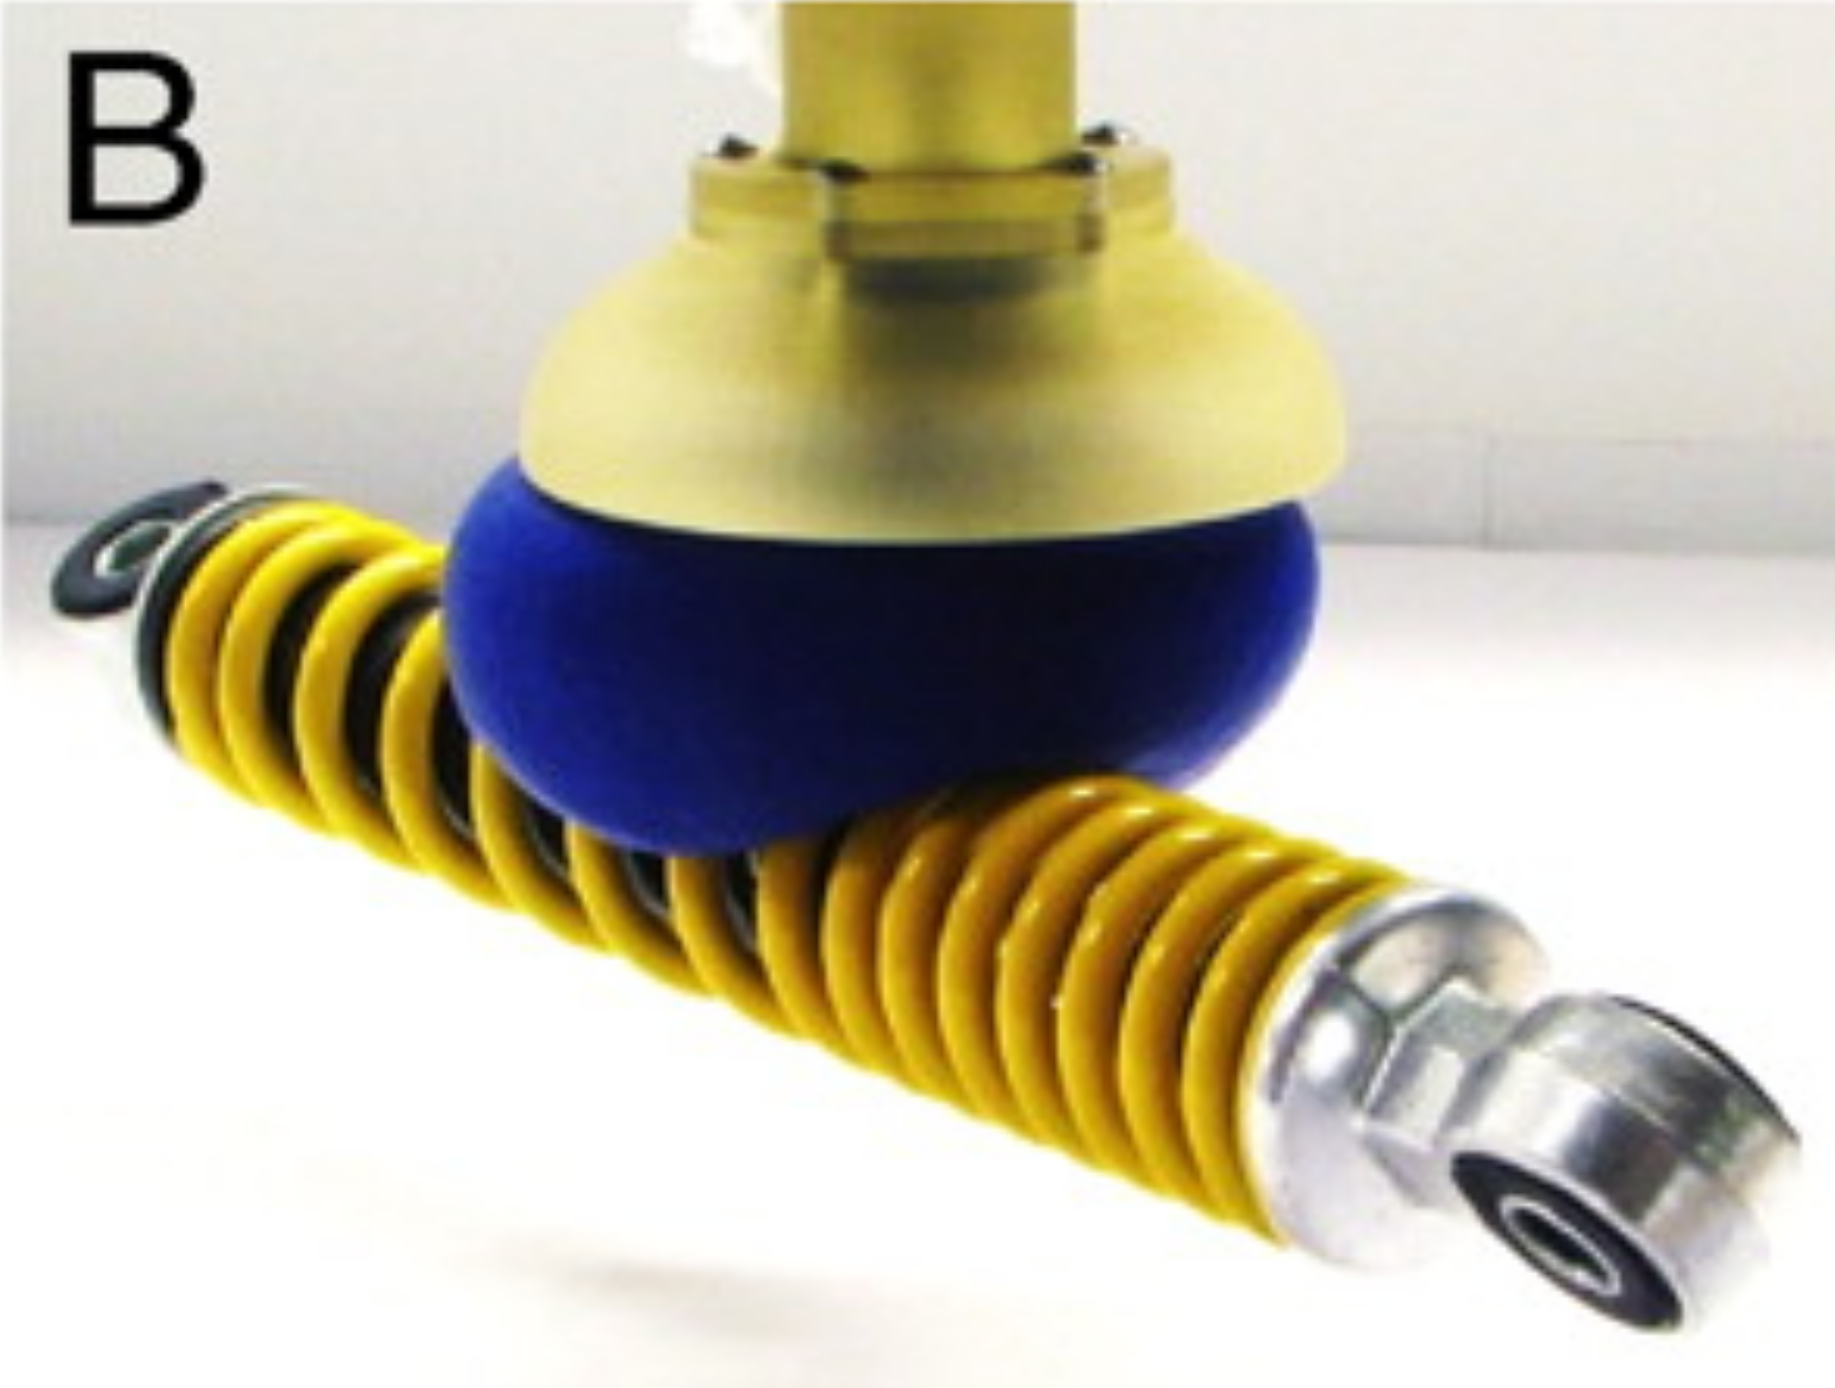
\includegraphics[width=0.7\textwidth]{Images/CoffeeBeanGripper.png}   
  %  
\includegraphics[width=.4\textwidth]{Images/placeholder.png}
        \caption[Coffee Bean Gripper]{Coffee Bean Gripper \cite{ParticleJamming}}
        \label{fig:Coffee Bean Gripper}
    \end{subfigure}
    \begin{subfigure}{.3\linewidth}
        \centering
    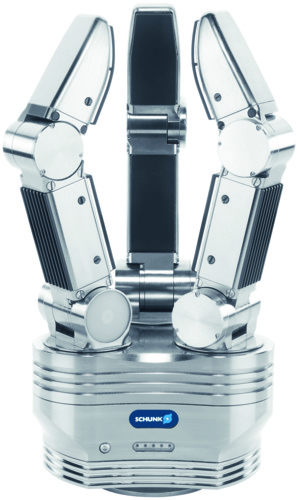
\includegraphics[width=0.7\textwidth]{Images/Schunk3FingeredGripper.jpg}
%         
\includegraphics[width=.4\textwidth]{Images/placeholder.png}
        \caption[Schunk 3 Fingered Gripper]{Schunk 3 Fingered Gripper \cite{Schunk3FingerGripper}}
        \label{fig:Schunk3FingeredGripper}
    \end{subfigure}
    \begin{subfigure}{.3\linewidth}
        \centering
        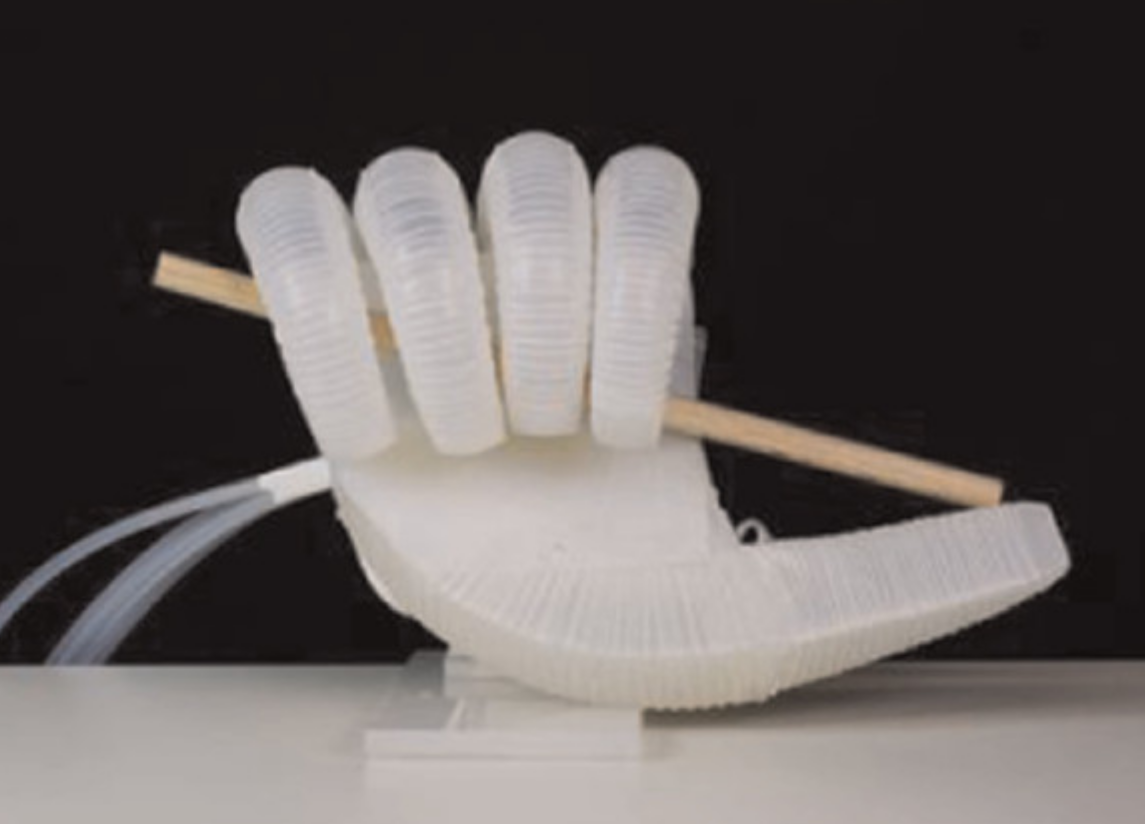
\includegraphics[width=0.7\textwidth]{Images/SoftRoboticGripper.png}
    %     
\includegraphics[width=.4\textwidth]{Images/placeholder.png}
        \caption[RBO Hand 2]{RBO Hand 2 \cite{RBOHand2}}
        \label{fig:RBOHand2}
    \end{subfigure}
\end{figure}

\section{Grasp Sensing}
Sensing is a vital part of any gripper and grasping motion. Without sensing, only highly structured tasks can be achieved. Sensing can typically be divided into two types, proprioceptive sensing and exteroceptive sensing. The former describes sensing which is used to measure physical information related to the current state of the system, i.e. joint angles, velocity, etc. This is critical to ensure that the robot behaviour is as expected, i.e. to use closed loop control. The latter refers to sensors which offer information about the target object or environment, i.e. force, pressure, temperature, etc. Exteroceptive sensing offers the ability to adapt to changes in its environment, to infer information about the object and environment and inform the actuation accordingly. Sensing is a fundamental building block of any general purpose gripping system. This section will examine some of the most common and most relevant types of sensing to grasping moving objects. 

\subsection{Image Sensing}

Autonomous robotic grasping and has always relied heavily on image sensors to provide the information needed to grasp the target object. Image sensing, both 2D and 3D, has many advantages over other types of sensing. It provides high resolution sensor data which can be collected in a non-intrusive way. Information about the object can be collected without physical interaction with the target object. For these reasons it has become the primary sensing mode used in manipulation and grasping tasks. Examples of the use of image sensors in grasping applications are present both in robotics research, and commercial products. Figure \ref{fig:RobotIQImageSensing} shows a commercial product with built in image sensing. All examples of grasping moving objects examined later in this chapter use image sensing. Furthermore. all robots participating in the 2018 Amazon Picking Challenge (APC)\cite{APCObservations} used image sensing, the use of image sensing in the 2018 APC is summarised in table \ref{table:APCSensorBreakdown}.

There are also difficulties associated with the use of image sensing. This type of sensing collects vast quantities of data, much of which is not relevant. Large amounts of computational power is required to filter and analyse the collected data to extract useful information. This becomes an important factor when grasping moving objects since the task is time critical. It is also a concern on robotic platforms which are computationally limited such as mobile platforms.

Robotic image sensing can generally be split into two distinct categories, 2 Dimensional (2D) and 3 Dimensional (3D) image sensing. Each is named for the type of data which it collects, ie. 2D image sensing refers sensors which collect is a 2D photograph of the scene whereas 3D image sensing collect 3D data about the environment, such the depth of an object, or the distant to a point. There is several ways in which depth information can be collected. The two most common are stereo camera pairs and depth cameras. Stereo pairs operate using the same mechanism as the human eyes. A pair of traditional 2D image sensors are placed a know distance apart. Using difference between the two images collected and basic geometry, depth information can be inferred. Depth cameras use a different mechanism, they project IR light patterns of a known structure onto the environment and extract depth information from how the patterns interfere with the scene. This mechanism is used in commercial depth cameras like the Microsoft Kinnect and Asus Xtion \cite{APCinhandproxandcontact}.

IR image sensing is a less commonly used form of image sensing. That being said, it is incredibly useful in certain applications. IR sensing is similar to traditional 2D image sensing with the exception that the sensor is sensitive to IR light rather than the visible spectrum. For this reason it can be very useful for interacting with humans since humans emit IR radiation allowing easy segmentation from their surroundings \cite{HumanIR}. IR image sensing is also used in manipulation, often for niche applications such as sorting and grading fruit based on ripeness \cite{MangoTest}, or assessing the integrity of power lines \cite{IRPowerLines}. One final use of IR image sensing in robotic manipulation is the use of IR reflectors as markers to simplify localisation. An example of this is the OptiTrack system \cite{OptiTrack} used by Seungsu Kim, et. al. to facilitate the grasping of tennis rackets and water bottle which are tossed at the robot \cite{TennisRacket}. These reflectors can be seen in Fig \ref{fig:IRMarkers}.

\begin{figure}
    \centering
    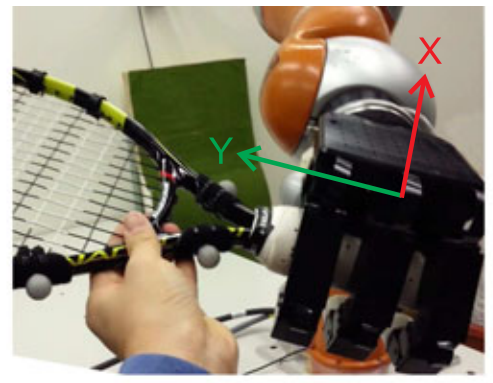
\includegraphics[width=.4\textwidth]{Images/CatchingObjectInFlight.png}
   % 
\includegraphics[width=.4\textwidth]{Images/placeholder.png}
    \caption{Dobot M1, soring and orientating chewing gum}
    \label{fig:IRMarkers}
\end{figure}

\begin{figure}
    \centering
       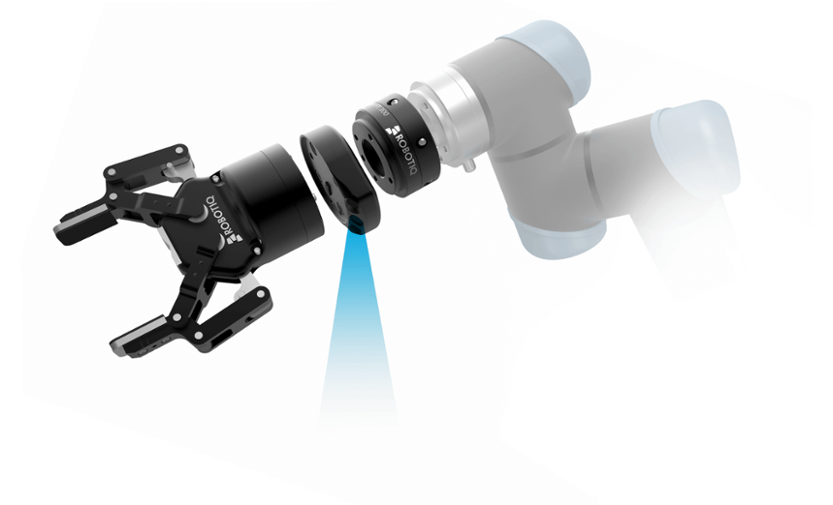
\includegraphics[width=0.4\textwidth]{Images/robotiq-vision-guided-robotic-hand-system.png}
%    
\includegraphics[width=.4\textwidth]{Images/placeholder.png}
    \caption[RobotIQ hand using image sensing]{RobotIQ hand using image sensing \cite{RobotIQVisionPic}}
    \label{fig:RobotIQImageSensing}
\end{figure}

\begin{table}[ht]
\begin{tabular}{|l|l|l|l|l|l|}
            & Head & Torso & End-effector & Arm & Total respondents\\  \hline
2D imaging  & 4    & 1     & 4            & 1   & 20 \\  
3D imaging  & 8    & 3     & 6            & 6  & 7  
\end{tabular}
\caption[Use of Image Sensing in the 2018 Amazon Picking Challenge]{Use of Image Sensing in the 2018 Amazon Picking Challenge, excerpt from \label{table:APCSensorBreakdown}
\cite{APCObservations}}
\end{table}

% Tactile Sensing
\subsection{Tactile Sensing}

Tactile sensing is a core component of how humans interact with and explore their environment. Experiments have shown how the loss of a ``sense of touch" is detrimental to a human's ability to grasp and manipulate objects \cite{HumanTactile}. Roboticists have long thought that endowing a robot with a ``sense of touch" would be beneficial, and perhaps necessary, to enable them to interact with an unstructured world \cite{iCub}. Tactile sensing is commonly used to detect collisions or contact points \cite{ConveyorBelt}. It can also be useful for understanding the nature of objects; it can help a system infer information about an object's properties like size, shape, weight, texture and temperature \cite{ObjectExploration,Vizzy,uSkinFingertip,InHandCP, TactileMango}, and can also be used to detect slip and shear between gripper and object \cite{First3DHall,HumanstoHumanoids,Survey}. It is therefore useful in object exploration \cite{TSiCub,BimanualExploration}, object classification \cite{James}, in-hand manipulation \cite{InHandCP} and grasping tasks \cite{Gifu}. 

Prior research has examined the nature of tactile sensing in more detail and rigorously categorised different types \cite{HumanstoHumanoids,TSdexterous}. For the purpose of this report we will summarise some of the commonly used types, and examine the advantages and disadvantages of different approaches. We will use the sensing mechanisms to categorise different approaches.


\begin{itemize}
    \item Hall Effect
    Tactile sensing based on the hall effect utilises a magnetic field to determine information about contact with an object. Typically in a hall effect based tactile sensor the position of a magnet relative to a hall effect sensor (a sensor which can measure the strength of a magnetic field) is in some way related to the current state of contact between the robot and an object. Therefore, details about the nature of contact , i.e. location, pressure, etc. can be inferred from reading the strength of the magnetic field. There are many example of such sensors in the literature, a recent example of this is uSkin \cite{uSkinFingertip} which has been applied and used in research to grippers such as the Allegro hand \cite{Allegro} and the iCub gripper \cite{iCub}
    \item Capactive
    Capactive tactile sensing uses the physical phenominium that the potential different between 2 conductors, separated by an insulator, is dependant on the distance between them. Using this, tactile sensors can use a soft, elastic material to act as the insulator between 2 conductors. In this way the capacitance will reflect the deformation of the elastic insulator and allow the robot to infer information about nature of contact with an object. 
    \item Pressure
    Pressure based tactile sensors also rely on an easily deformable, elastic material. In this case a pressure sensor (barometer) measures the pressure of the material. This pressure will respond in a predictable way to contact forces on the material, representing contact between the robot and an object.
\end{itemize}


\subsection{Joint Feedback}
Joint Feedback is our first example of proprioceptive sensing, enabling the robot to monitor the position of each of its joints and therefore extrapolate its own position in space. This type of sensing is essential for control purposes, i.e. to provide feedback to the motor controller to ensure that the desired motion is achieved. There are many different mechanisms which can be used to provide joint feedback and there are examples of each being implemented on in robotics applications. These are discussed below.
\begin{itemize}
    \item Magnetic Encoders
    Magnet encoders also rely on the hall effect, and are used to monitor the position of a shaft. The relative orientation of two parts of the robotic system is monitored by attaching a magnet to one and a hall effect sensor to the other. The magnetic field measured is dependant on their relative orientations and the position of the joint can therefore be inferred.
    \item Optical Encoders
    Optical encoders measure relative rotation between two parts of a robotic system. Unlike magnetic encoderes they do not measure in absolute terms but monitor the relative movement of a shaft. A disc with a pattern of slits in attached to the rotating shaft, an IR emitter is place on 1 side of the disc and a receiver is placed on the other. The pattern of flashes, caused by the slits aligning with the emitter and detected by the receiver can be analysised to give information about the rotation. 
    \item Mechanical Encoders
    Mechanical encoders use a similar mechanism as optical encodes and attach a disc with a custom pattern to the rotating shaft. In this case it is mechanical contacts which interacts with the disc and produce an electrical signature representative of the movement of the shaft.
    \item Potentiometer
    Finally, potentiometers or variable resistors can be used to sense joint position. The potentiometer used in this application generally has a resistance determined by the relative orientation of an internal shaft to the rest of the sensor. By coupling this internal shaft to a joint shaft the joint angle can be measured. A draw back of this type of joint sensor is that the variable resistor will have some maximum and minimum resistance which it can achieve and is therefore unsuitable for measuring contineous rotation. In reality potentiometers either have a finite angle of rotation or have a discontinuity in their resistance at some angle. This is generally not a problem for robotic gripper or manipulator joints which also tend to have a finite joint angle range and don't require contineous rotation.
\end{itemize}

\subsection{Misc Sensors}

There a huge number of sensors which have previously been implemented in robotic systems, however it is outside the scope of this document to complete a full review. There are some other, less common, examples which are particularly relevant to this research and so will be mentioned here. Although depth cameras have been mentioned, there are a range of other types of range finding sensors which have been implemented in robotic gripper systems. A more niche example is the work of Ilhan Konukseven et. al. \cite{FingertipEmitterReceiverMovingObjectII, FingertipEmitterReceiverMovingObject}. In this research a custom sensor is developed to calculate an error in alignment between the axis of the gripper and the axis of symmetry of the object to aid in grasp alignment. Whisker-like sensors, inspired by whiskers on animals, have also been explored in robotics as a way of exploring unknown environments \cite{2000Konukseven}. The use of whisker sensors have been explored on wheeled robots for close wall following \cite{CloseWallFollowing} and in manipulation for object localisation, recognition and grasping \cite{TactilePerception}.


\section{Actuation}\label{Actuation}
Actuation is a fundamental part of any manipulation system, actuators are the components which enable a system to move. At a very high level the actuator will take some energy input, usually in the form of electrical or potential energy and convert it to kinetic energy. In the manipulation context, actuators are essential both for moving the end effector into position and to enable the end effector to grasp the object. This research is most concerned with the motion which grasps the object however similar actuators are used in all areas of robotics. This section will look at the most common actuators used in robotic grippers to date, the advantages and disadvantages, the trade off and the applications. This section will also examine actuation strategies and the advantages and disadvantages of underactuated systems compared to fully actuated systems.

The first method of actuation discussed is the DC motor. A simple system where an electric potential input will cause a shaft to rotate. They are effective in a large range of sizes. They are inexpensive and efficient, making them the most commonly used method of actuating any part of a robot. Despite this there are several disadvantages. DC motor produce maximum power and are most efficient at high speeds, this results in the use of gears and other motion transmission methods which reduce the speed while increasing the torque. Although this trade off, more torque for less speed, is advantageous for robotic applications there are inefficiencies and errors associated with these devices. Friction, noise and backlash are all problems which are introduced while making the system more expensive. Backlash in particular is a problem for robotic manipulation. In order to maximize the number of poses which the manipulator can position and orientate its end effector in, a manipulator generally has a large number of Degrees of Freedom (DOF). Similarly to maximise the flexibility of a gripper it also has a large number of DOF. In both cases these DOF are arranged in a relatively long open kinematic chain. The effect that blacklash and any other error between the desired and actual joint angle is that these errors propagate and accumulate through the chain such that small relative errors caused by backlash at each joint causes a large absolute error in the position of the end effector.

%% Potentially a nice Diagram of error propagation

A further disadvantage of using simple DC motors is the absence of a feedback mechanism. Generally the speed of a DC motor is determined by the voltage applied (neglecting the back emf in its coil) and the output torque is proportional to the current. Due to variations in these parameters and the effects of a load on the shaft it is difficult to determine the position of the motor at any particular time, based on the inputs to the motor. Furthermore using the inputs to a DC motor as a way of determining the position of a robot joint is subject to error propagation since the voltage input determines speed and in robotic manipulation we are generally interested in joint position. For example a small error in the estimation of the motor speed would cause an ever growing error in the joint position over time. For this reason, simple DC motors are almost always implemented with an separate feedback mechanism.

Stepper Motors are another common method of actuation in robotics and one which addresses this problem. They are similar in some ways to a simple DC motor but overcome some of the challenges while introducing its own challenges. Like a simple DC motor a stepper motor takes DC electricity as an input and produces kinetic energy in the form of a rotating shaft. The internal differences between a simple DC motor and a stepper motor are outside the scope of this document but in effect the mechanism by which a stepper motor operates allows position controlled unlike a speed controlled simple DC motor. This ability to control the position of the motor comes at the cost of requiring logic to control the motor, generally in the form of a micro-controller. Steppers motors also exhibit holding torque, a feature which other DC motors lack. A stepper motor can hold its shaft in position opposing external forces. This is often useful in manipulation applications.

Motors are the most common form of actuation in robotics, and the form using in this project however other types of actuation include piezo electrics, pneumatics and hydraulics. Each with its own set of advantages and drawbacks. These will not be discussed in this document.

\subsection{Under Actuation}\label{UnderActuaction}

Underactuation is a technique often used in robotics, among the mostly commonly cited reasons for choosing to underactuate a system is to reduce the number of actuators required \cite{UnderactuationReductionInActuactors}, to simplify the control and therefore computational overhead and to fully take advantage of the system's natural dynamic characteristics \cite{PassiveDynamicWalker}. A system is said to be underactuated if the number of dimensions in which it is free to move, i.e. its Degrees of Freedom (DOF) is more than the number of independently actuated joints. Most robots can be described by 

\begin{equation}
\ddot{q} = f_1(q,\dot{q},t) + f_2(q, \dot{q},t)u   
\end{equation}
where \(u\) is the control vector, \(t\) is time and the robot's state can be described by a vector of positions (\(q\)) and velocities(\(\dot{q}\)). In this more mathmatical formulation if 
\begin{equation}
    rank[f_2(q,\dot{q},t)] < dim[q]
\end{equation}
then the system is said to be underactuated.

More specific to robotic grippers underactuation can often be a desirable quality and give the grasper the ability to self adapt to object geometry. The use of elastic or flexible material to mechanically couple joints in the finger can allow the gripper to better adapt to the shape of an object and increase the chances of a successful grasp simply by carefully designing and utilising the physical embodiment of the hand.

However it has been found that underactuation tends to hinder grasper dexterity \cite{RBOHand2}. Using this method inheriently, forfeits independent control over each joint individually. That being said, through tuning the moments and elastic elements at each joint the order in which the joints act, when the finger is actuated, can be controlled. The most common use of this, shown in figure \ref{UnderActuaction}, is to ensure that greatest turning moment, when actuated, is about the bottom joint. This will turn until it encounters an object. Typically the next largest turning moment would be the middle joint, which similarly rotates until it meets the object. Finally, the smallest turning moment is on the joint for the tip of the finger which completes the grasp.

\begin{figure}

    \centering
    \begin{subfigure}{.3\linewidth}
        \centering
%    
\includegraphics[width=.4\textwidth]{Images/placeholder.png}       
    
\includegraphics[width=0.7\textwidth]{Images/Underactuaction/FullyOpen.png}
        \caption{Fully Open}
        \label{fig:UAFullyOpen}
    \end{subfigure}
    \begin{subfigure}{.3\linewidth}
        \centering
        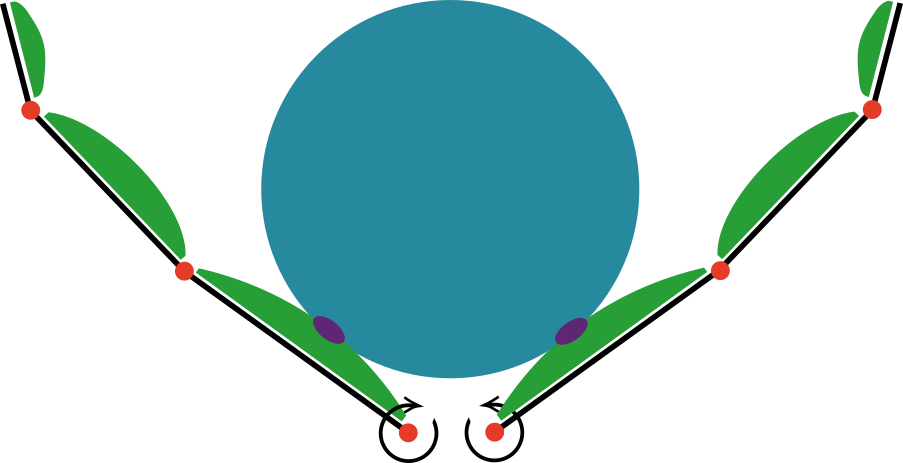
\includegraphics[width=0.7\textwidth]{Images/Underactuaction/phase1png.png}
 %  
\includegraphics[width=.4\textwidth]{Images/placeholder.png}
        \caption{Step 1, Bottom phalanx rotates and makes contact}
        \label{fig:UAStep1}
    \end{subfigure}
    \begin{subfigure}{.3\linewidth}
        \centering
 %   
\includegraphics[width=.4\textwidth]{Images/placeholder.png}                   
    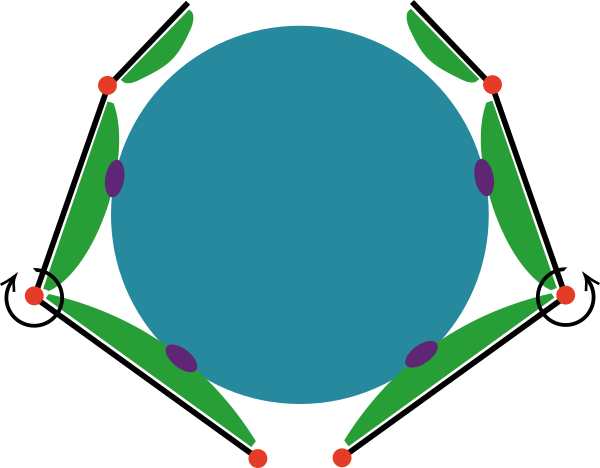
\includegraphics[width=0.7\textwidth]{Images/Underactuaction/phase2.png}
        \caption{Step 2, Middle phalanx rotates and makes contact}
        \label{fig:UAStep2}
    \end{subfigure}
    \begin{subfigure}{.3\linewidth}
        \centering
        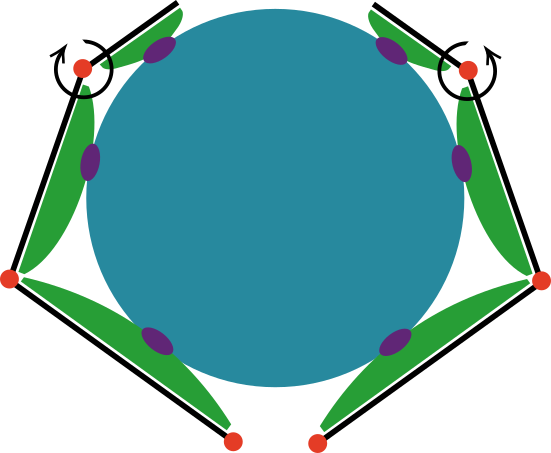
\includegraphics[width=0.7\textwidth]{Images/Underactuaction/FullyClosed.png}         
%    
\includegraphics[width=.4\textwidth]{Images/placeholder.png} 
        \caption{Step 3, Top phalanx rotates and makes contact. Fully Closed}
        \label{fig:UAStep3}
    \end{subfigure}
    \caption{Basic concept of underactuation}
    \label{fig:UnderActucation}
\end{figure}

\section{Planning vs Reactive Grasping Strategies}

Literature reflecting on the Amazon Picking Challange (APC) 2015 \cite{Eppner2018} proposes that the development of a robotic system can be described on 4 different spectra. Modularity verus integration, generality vs assumptions, computation versus embodiment and planning versus feedback. It is the last of these which is most relevant when discussing grasping strategies.

A fully planning based control strategy adheres strictly to a sense-plan-act structure. Manipulation and grasping is oblivious to sensor stimulus after the sense stage. This approach to grasping requires a static, controlled and structured environment. The opposite is a strategy based wholly on feedback with no high level planning. Instead all actuation is directly caused by sensor stimulus in real time. This type of strategy, while adaptable to changes in the environment, makes it very difficult to complete high level, complex tasks.

%aworld model, leading to verifiable solutions. Feedback from physical interactions, on the other hand, reduces uncertainty and allows to find local solutions without expensive compu- tation. We thus suggest to use planning only when necessary and explore the use of feedback as an alternative when the manipulation task does not require global search."  Feedback is identified as a way to grasp objects which are typically more difficult to grasp. It is identified as something which can be used to combat picking wrong objects, smaller objects, objects which move, the shelf moving. "Manipulation tasks in particular can be gratly simplified by exploiting feedback from contact with the environment""Feedback approaches are particularly useful in the presence of uncertainty, high dimensionality, long time horizons and inaccurate models""Planning would be time-consuming, computationally demanding"

An effective way to examine current state of the art in grasping strategies is to examine approachs taken in robotic competitions. The robotics community often poses challanges and encourages research in particular areas through robotics competitions. Examples of these include RoboCup, RocKIn, and the Amazon Picking Challange (APC). These competitions and the tasks set by them are often used as benchmarks for the performance of different robotic systems and approaches \cite{CompetitionsAsBenchmarks}. The concensis from reflections on these competitions are that although both planning stragtegies, as used by the Delft team in 2016 \cite{Delft}, and reactive strageties, as used by team RBO in 2015, have their strengths, they both won the competition in their respective years, a hybrid control strategy is a more effective solution for robotic gripper \cite{APCObservations}.

\section{Computation}
A common problem which arises in moving object grasping is the high computational overhead associated with a heavy reliance on machine vision and motion planning techniques\cite{KinematicallyOptimal,Eppner2018}. As an example, research conducted by Berthold et al. (2010) \cite{KinematicallyOptimal} used optimised parallel computational loads spread across 32CPU cores in order to perform real-time optimisations for catching a flying ball. Despite advances in computer architectures and software optimisation since that research, the problem of high computational effort remains a significant one. 

Precision is also a major limiting factor for approaches based on only on vision sensors. It is reiterated throughout the literature that "high precision in space and time" is one of the greatest challenges for catching a ball thrown in three dimensional space \cite{RollinJustin}. In that particular example the estimate of the interception position and time need to be accurate within 2cm and 5ms.


\section{Grasping Moving Objects}

Dynamic objects adds another significant challenge to the manipulation problem. Robotic interaction with moving objects has long been a topic of research in robotics\cite{Buhler1989, 1991BallTracking}. Previous research shows robots grasping \cite{ConveyorBeltTracking, ConveyorUnknownObject}, catching \cite{TennisRacket, RollinJustin, DisneyRobot, HandEye, CatchingSoftly}, batting \cite{Muelling2014, Senoo2006} and juggling \cite{JugglingWithKitchenFunnels, Buhler1989, OneHandedJuggling}. These abilities enabled a range of new robotic applications this will be discussed below.

\begin{itemize}
    \item Games and Sports
    
    Much of the research to date which examines how robots could interact with moving objects involve enabling a robot to participate in a sports activities. One of the earliest examples of research in this area is using robots to play ping-pong \cite{Anderson1989}. This area of research has been very active since and there has been continuous improvements have been made \cite{Koc2018}. Other examples of research endowing robots with the ability to play games or sport include Soccer \cite{RoboCupSoccer}, Kendama \cite{Kendama}, Ice Hockey \cite{IceHockey} and Air Hockey \cite{AirHockey}. Both soccer and hockey have been facilitated by Robocup. Robocup is an international robotics competition in which teams of robots compete against each other. Research inspired or guided by these competitions has lead to advancements in robotic design, computer vision, multi-agent systems and many other robotic fields including interaction with dynamic objects \cite{RoboCupSoccer, FuzzyRobocup}. 
    
\cite{RoboCupSoccer}.
    
    \item Human Robot Interaction
    
    The ability to grasp a moving object is also used to as a means of allowing humans to interact with robots. Disney designed a system which could operate in a theme park and could interact which visitors. Identifying contact based human-robot interaction as a potential safety issue, a robot which could play catch was developed \cite{DisneyRobot}. Playing catch as a means to interact with a robot is not a concept unique to Disney. Other research has identified playing catch as a "simple, safe, and fun way" to interact with a robot \cite{JugglingWithKitchenFunnels}.
    
    \item Operating in an unstructured environment
    
    Investigating the autonomous grasping of moving object doesn't always map to a use case where the developed ability can be directly applied. Much of the literature identifies the grasping moving objects as a way to address challenges which are associated with deploying robots in unstructured environments. Grasping or otherwise interacting with a moving objects is a complex task which has demanding temporal and spacial constraints \cite{Anderson1989, EarlyAnticipation}. Investigating the grasping of moving objects has enabled the exploration of novel trajectory generators \cite{Senoo2006, Lampariello2011}, sensor-based reactive motion \cite{Senoo2006} and energy optimisation \cite{Lampariello2011} to name a few . These are explored in the context of a ball catching use case but can be applied more generally to enable robots to operate in unstructured environments 
\end{itemize}


Since this research focuses on grasping we can categorise the most relevant examples to date into four different levels of increasing difficulty based on the behaviour of the target object.

\begin{enumerate}
    \item Regular Object, controlled trajectory see Fig. \ref{fig:ConvBelt}
    \item Irregular object, controlled trajectory see Fig. \ref{fig:MilkConvy}
    \item Regular object, uncontrolled trajectory see Fig.\ref{fig:DisneyBot}
    \item Irregular object, uncontrolled trajectory see Fig. \ref{fig:TennisRacket} 
\end{enumerate}

\begin{figure}
    \centering
    \begin{subfigure}{.4\linewidth}
        \centering
        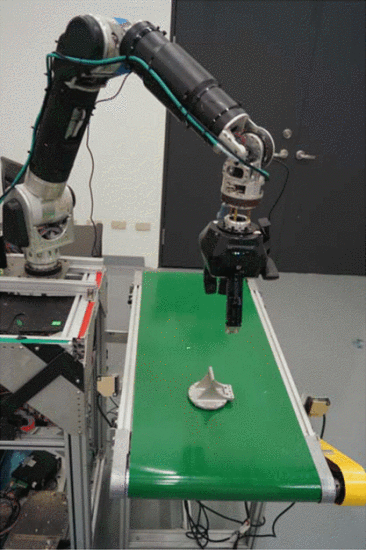
\includegraphics[width=.8\textwidth]{Images/ConveyorBelt.png}
%    
\includegraphics[width=.4\textwidth]{Images/placeholder.png}
        \caption[Category 1: Machined Part on a Conveyor Belt]{Category 1: Machined Part on a Conveyor Belt \cite{ConveyorBeltTracking}}
        \label{fig:ConvBelt}
    \end{subfigure}
    \begin{subfigure}{.5\linewidth}
        \centering
        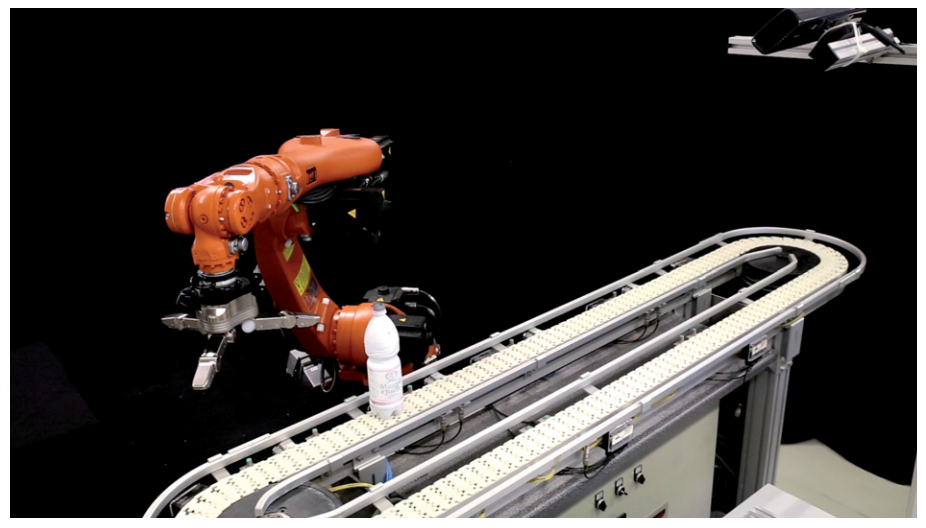
\includegraphics[width=.8\textwidth]{Images/ConveyorUnknown.png}
%    
\includegraphics[width=.4\textwidth]{Images/placeholder.png}
       \caption[Category 2: Grasping an Unknown Object on a Conveyor Belt]{Category 2: Grasping an Unknown Object on a Conveyor Belt \cite{ConveyorUnknownObject}}
        \label{fig:MilkConvy}
    \end{subfigure}
    \begin{subfigure}{.4\linewidth}
        \centering
        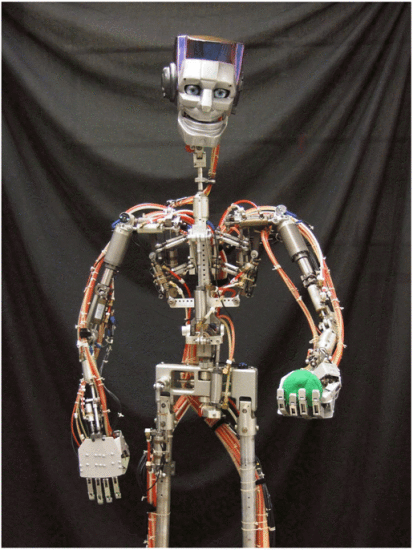
\includegraphics[width=.8\textwidth]{Images/Disney.png}
%    
\includegraphics[width=.4\textwidth]{Images/placeholder.png}
        \caption[Category 3: Theme Park Juggling Robot by Disney]{Category 3: Theme Park Juggling Robot by Disney \cite{DisneyRobot}}
        \label{fig:DisneyBot}
    \end{subfigure}
    \begin{subfigure}{.5\linewidth}
        \centering
    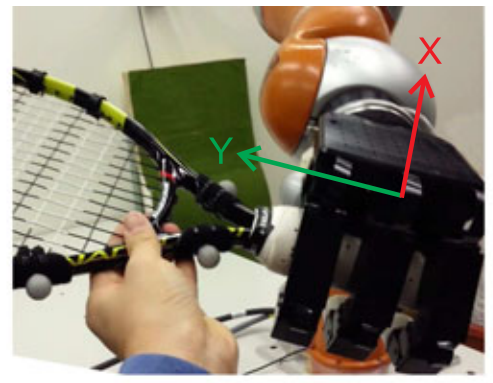
\includegraphics[width=.8\textwidth]{Images/CatchingObjectInFlight.png}
        \caption[Category 4: Catching a Thrown Tennis Racket]{Category 4: Catching a Thrown Tennis Racket \cite{DisneyRobot}}
        \label{fig:TennisRacket}
    \end{subfigure}
\end{figure}

Grasping or otherwise interacting with a moving object is something that is often applied in automation applications to increase the efficiency and throughput of automated process. Potential situations where it might be necessary to grasp a moving object include visual quality checks of finished parts or as shown in \ref{fig:SortingChewingGum} sorting and/or regularising the orientation of objects on an assembly line. For this reason, a common application where a robot may be required to grasp a moving object is when the object is on a conveyor belt \cite{ConveyorBeltTracking, FingertipEmitterReceiverMovingObjectII,FingertipEmitterReceiverMovingObject}; there are even examples of tactile sensing being used to inform a grasp during manipulation of an object on a conveyor belt \cite{ConveyorUnknownObject}. The context in which these robots are operating is very different from the unstructured scenarios of everyday life; objects are moving at a relatively slow, constant, speed, making them much easier to localise, predict their behaviour, and subsequently grasp them.

\begin{figure}
    \centering
    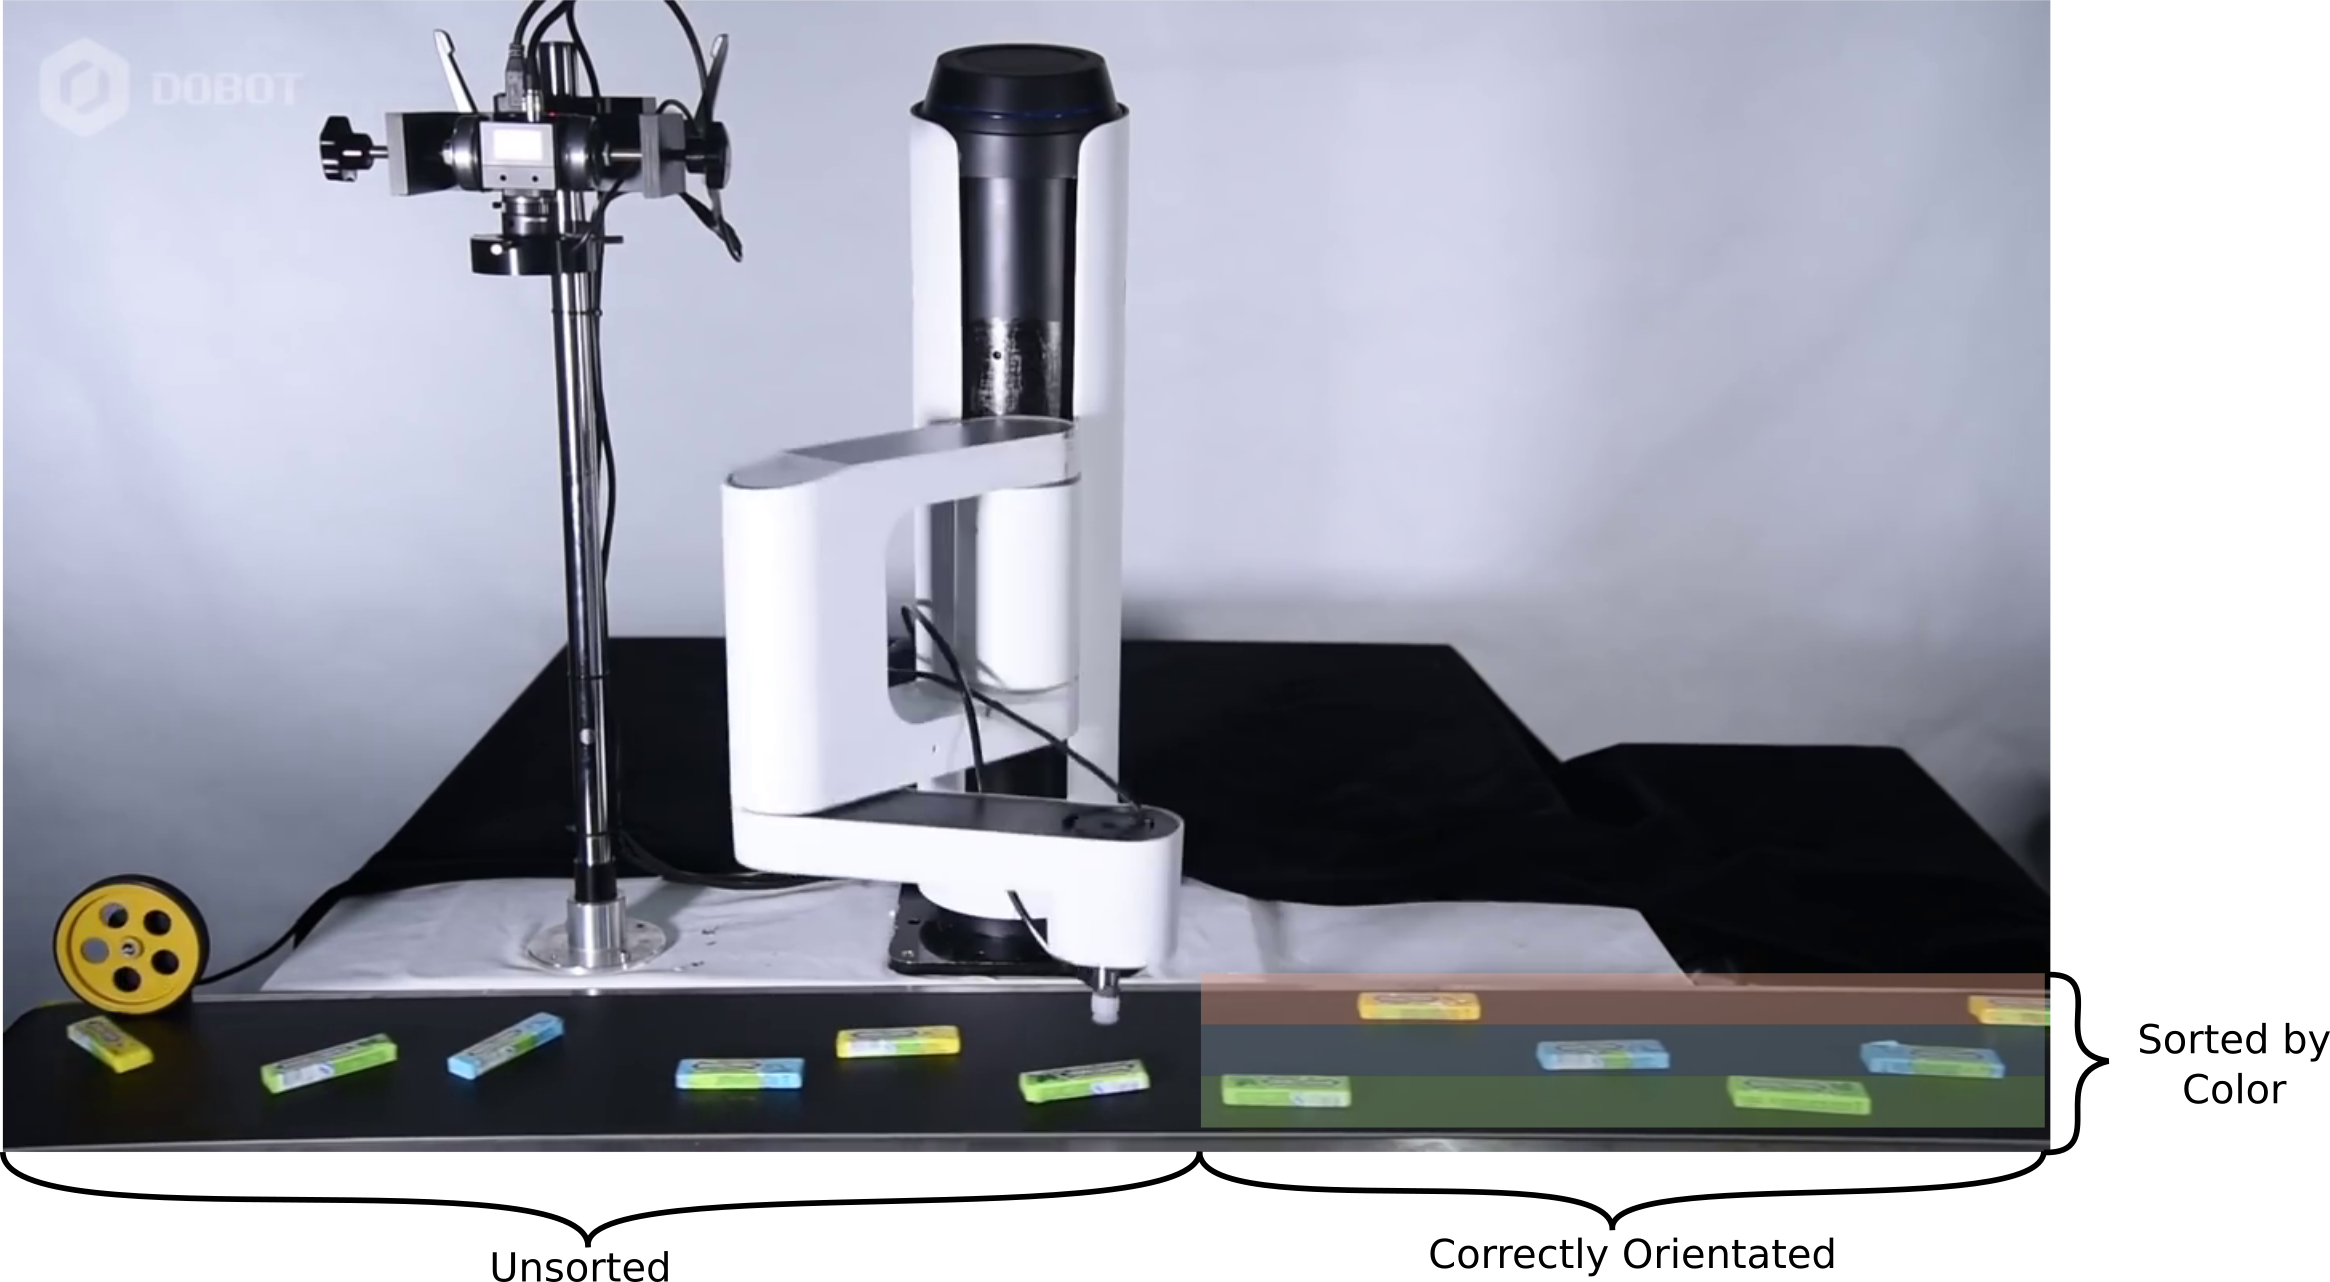
\includegraphics[width=.4\textwidth]{Images/Sorting.png}
%    
\includegraphics[width=.4\textwidth]{Images/placeholder.png}
    \caption{Dobot M1, soring and orientating chewing gum}
    \label{fig:SortingChewingGum}
\end{figure}

The grasping task becomes more complex with the complexity of the obejct geometry. When grasping simple cuboids, such as the chewing gum example, the grasping task is relatively simple. This is more difficult when grasping objects such as bottles, cups and pitchers \cite{ConveyorUnknownObject}. In this particular example tactile sensing is used to inform the grasp however the object is on a conveyor belt and its speed is therefore known and constant.

In these example the location and speed of the object was known, typically because the object was on a conveyor belt. Although more challenging than grasping static objects, these problems can effectively be simplified to grasping a static object by matching the velocity of the target object in the axis of movement during the grasp \cite{FingertipEmitterReceiverMovingObjectII,FingertipEmitterReceiverMovingObject}. When the movement of the object is less controlled the problem complexity increases again. An example of this which has long been an active research area spherical objects which have been thrown through the air at the robot \cite{1991BallTracking}. Spherical objects are common in research concerned with the grasping of moving objects in non-structured domains \cite{DisneyRobot,RollinJustin,EarlyAnticipation}. These objects are well suited to moving object grasping as they present the same grasping problem regardless of orientation. 

An example of this, already mentioned above, is the disney created robot, designed to work in theme parks. Developed as an attraction for park visitors, who could interact with the robot without being physically close or needing to contact the robot which was considered a safety concern. The robot could catch a ball which was thrown to it and would throw the ball back to the user. The approach taken massively simplified the grasping motion of the fingers by using a soft ball and foam extension to the gripper to increase the area of the hand and therefore the interception area which would result in a successful grasp. Rollin Justin has also been applied to a ball catching problem, in this case the robot could catch two balls that were thrown simultaneously. In order to achieve this a high number of degrees of freedom were needed, not just the arms but the torso and the mobile platform itself. Both of these examples focus solely on vision sensors to locate and track the object. An estimation of an interception position and time was then used to move the gripper into the correct position and orientation. Neither example examined the closing motion of the gripper, opting instead to close the fingers when the estimation suggested the target object was in the optimum location. 

The final level of complexity for which examples can be seen in the research are successful attempts to dynamically grasp objects with complex geometries, these include tennis rackets and water bottles \cite{TennisRacket}. In this example the additional complexity is addressed by emplying more advanced (local and distributed) vision sensing, deep learning and a programming by demonstration approach \cite{TennisRacket}.

In all these examples, the focus of the research is on the vision system, which predicts an intercept position and time, or the mechanical system and achieving the intercept position within a short time window. They have largely ignored (or simplified) the interaction between the gripper and object. For example in the Kendama study \cite{Kendama}, the robot has a bespoke end-effector for catching the ball without the need for a grasp, the Disney gripper \cite{DisneyRobot} uses a foam rim to simplify catching. A more comprehensive review of how research to date has simplified the grasping motion is outlined in section \ref{GraspingMotion}.

\subsection{Grasping Motion}\label{GraspingMotion}

The area of interest for this project is the grasping motion itself, grasping motion in this context specifically refers to the motion of the gripper and fingers as they interact with the object. Many of the examples of the autonomous grasping of moving objects given above focus on either the calculation of an appropriate interception position and time or the ability of the robot to move into position sufficiently quickly. There is a lack of research about, and therefore understanding of, the optimum grasping motion since typically this part of the problem is simplified to a rapid closing of the fingers \cite{RollinJustin, KinematicallyOptimal} or by using solutions like kitchen funnels \cite{EarlyAnticipation}, and foam \cite{DisneyRobot} to remove the need for a robust grasp. Table \ref{Simplifications} shows a history of research concerned with the grasping of moving objects. It demonstrates how the complexity of the motion of the gripper itself if generally abstracted so as to investigate other parameters.

\begin{table}[ht]
\begin{tabular}{|l|l|l|l|l|}
\hline
\textbf{Robot}& \textbf{Year} & \textbf{End Effector} & \textbf{Dimensions} & \textbf{ref} \\ \hline

\begin{tabular}[c]{@{}l@{}}Four DOF, Cable\\ Driven Arm\end{tabular}& 1991 & \begin{tabular}[c]{@{}l@{}}None, Tracking\\ Only \end{tabular} & N/A & \cite{1991BallTracking} \\ \hline

DLR robotic arm & 2001 & "Net" & \diameter160mm & \cite{2001OffTheShelf} \\ \hline

Humanoid Robot & 2002 & \begin{tabular}[c]{@{}l@{}}Kitchen Funnels and \\ Baseball Glove \end{tabular} & Unknown & \cite{JugglingWithKitchenFunnels} \\ \hline

Saika Robto & 2002 & "Cooking Basket" & \diameter120mm & \cite{Saika} \\ \hline

\begin{tabular}[c]{@{}l@{}}Whole Arm\\ Manipulator \end{tabular} & 2005 & \begin{tabular}[c]{@{}l@{}}"{[}T{]}hree DOF\\ end effector"\end{tabular} & Unknown & \cite{HandEye} \\ \hline

6-DOF COTS Arm & 2007 & Cardboard Basket & \diameter 140mm & \cite{COTS} \\ \hline

DLR-LWR-III arm & 2010 & DLR-Hand-II & Unknown & \cite{KinematicallyOptimal} \\ \hline

Rollin' Justin & 2011 & \begin{tabular}[c]{@{}l@{}}12 DOF, DLR-Hand-II \\ see Fig. \ref{fig:RollingJustinHand} \end{tabular} & $ \approx  140mm^2 $ & \cite{RollinJustin} \\ \hline

\begin{tabular}[c]{@{}l@{}}Sky, a Disney \\ Humanoid Robot\end{tabular} & 2012 & \begin{tabular}[c]{@{}l@{}}Humanoid Gripper, "augmented\\ ...{[}by{]} a foam rim to provide a \\ more cup-like shape suitable for\\ catching" see Fig. \ref{fig:DisneyFoam} \end{tabular} & \begin{tabular}[c]{@{}l@{}} $ 100mm^2 $ \\ $ + foam $ \end{tabular} & \cite{DisneyRobot} \\ \hline

Kuka LWR4+ & 2014 & 16-DOF Allegro Hand & Unknown & \cite{TennisRacket} \\ \hline

\end{tabular}
\caption{End effectors used to grasp moving objects}
\label{Simplifications}
\end{table}

\begin{figure}
    \centering
    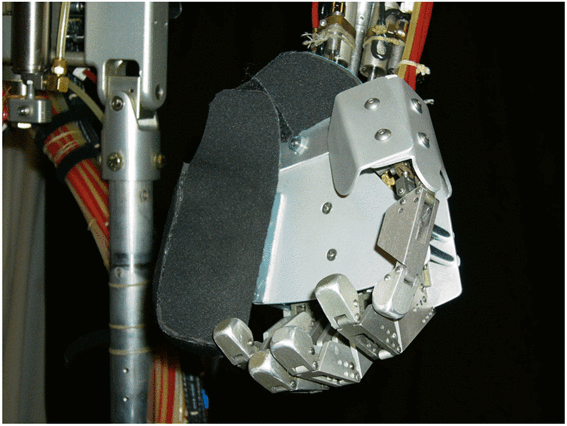
\includegraphics[width=.4\textwidth]{Images/DisneyFoam.png}
%    
\includegraphics[width=.4\textwidth]{Images/placeholder.png}
    \caption{Foam Augmentation to the Disney hand to facilitate grasping \cite{DisneyRobot}}
    \label{fig:DisneyFoam}
\end{figure}
\begin{figure}
    \centering
    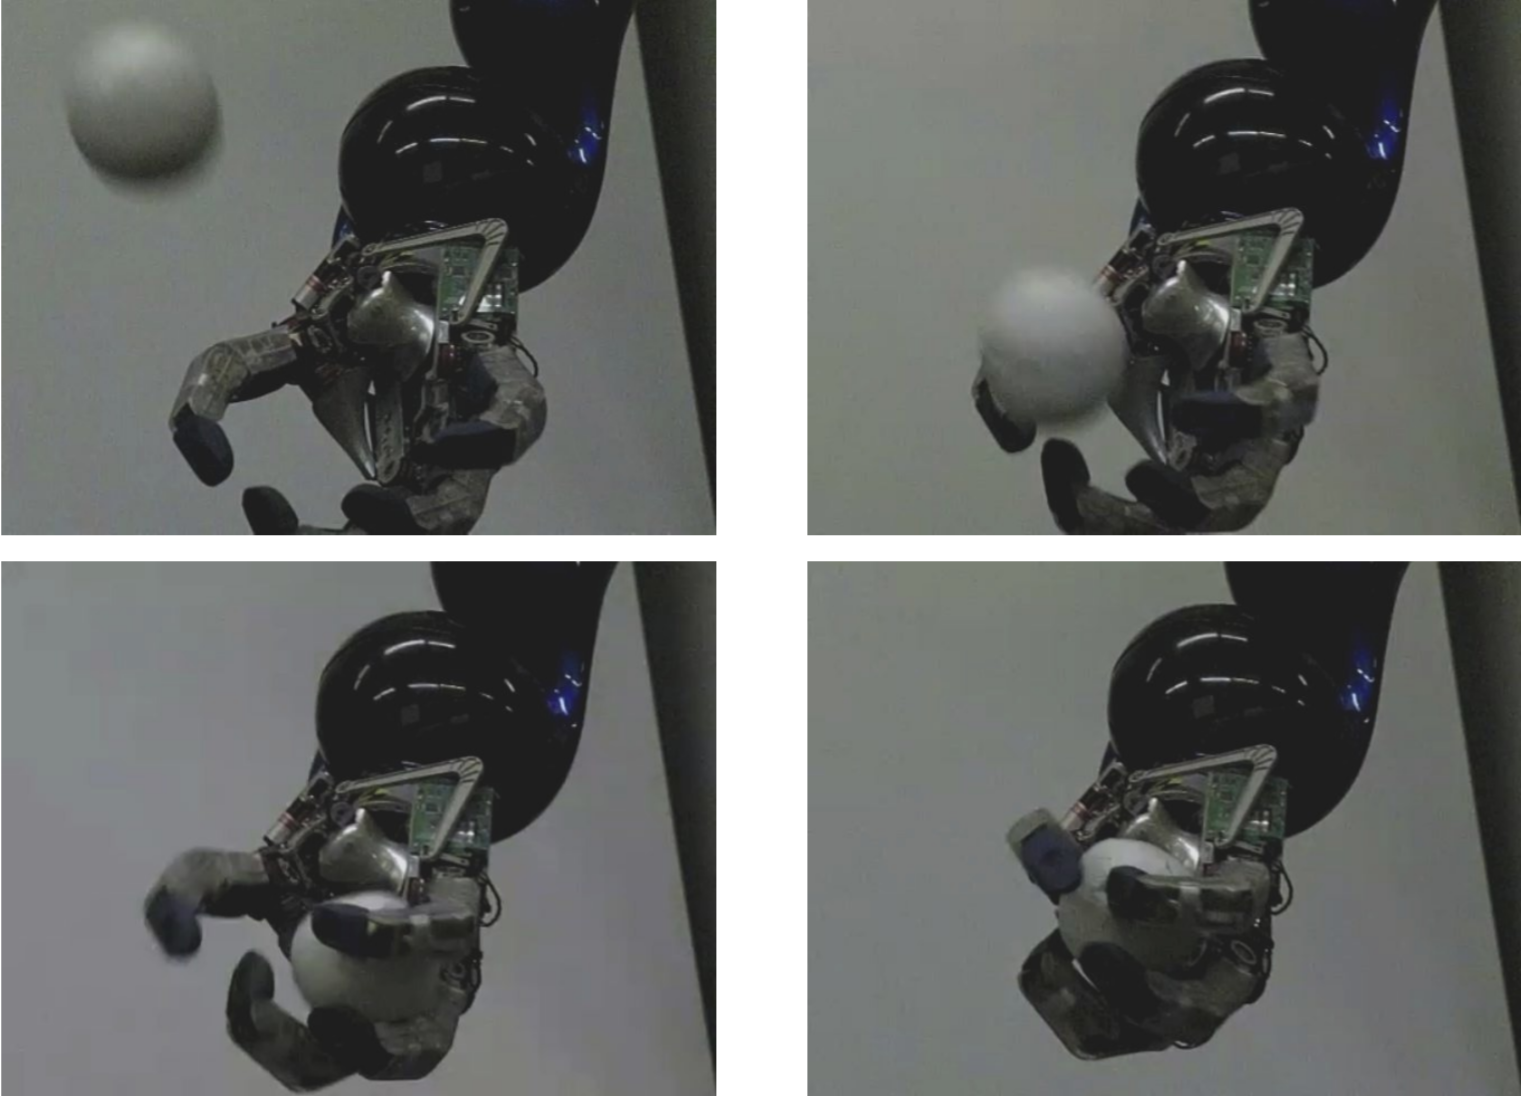
\includegraphics[width=.4\textwidth]{Images/RollingJustinHand.png}
%    
\includegraphics[width=.4\textwidth]{Images/placeholder.png}
    \caption{DLR-II Hand used on Rollin Justin \cite{RollinJustin}}
    \label{fig:RollingJustinHand}
\end{figure}
\begin{figure}
    \centering
    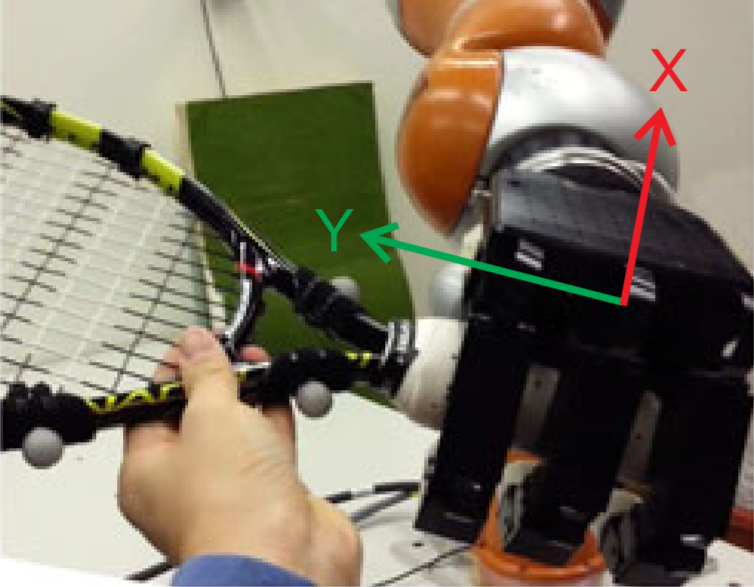
\includegraphics[width=.4\textwidth]{Images/VisionMarkersTennisRacket.png}
 %   
\includegraphics[width=.4\textwidth]{Images/placeholder.png}
    \caption{Vision Markers used to simplify tracking \cite{TennisRacket}}
    \label{fig:VisionMarkersTennis}
\end{figure}

Coupled dyamical system - talks about finger position., focuses on finger apature based on studies of human grasps. Reach is in reach-grasp senarios where perbutions are introduced mid reach and grasp. \cite{Shukla2012}


\section{Research Contribution}
In a survey conducted on competitors in the 2015 Amazon Picking Challenge \cite{APCObservations}, the introduction of reactive control was was the dominant response from participants when ask to reflect on what changes they would make to their system. In the same survey 84\% of respondents agreed with the statement that "Perception needs to be better integrated with motion planning" and 68\% agree that "Motion planning needs to be better integrated with reactive planning". This study concluded that "the use of reactive control to compensate for inaccurate sensing and actuation of an underlying deliberative architecture appears to be powerful". This sentiment is echoed throughout the literature, sensory feedback is said to be a necessity in order to robustly perform high soeed tasks \cite{Senoo2006}. Despite this apparent agreement amongst researchers on the need for reactive control based on sensory input this review of the existing literature has found that the contribution of sensing in grasping moving objects is a under-explored area, this project aims to tackle this.


%\section{Tactile Servoing}
%There are many examples of tactile sensing being used to inform and control the motion of a robotic gripper referred to as tactile servoing. The initial concept for tactile servoing proposes that the progress of a manipulation task can be observed and monitored through the sensor data from embedded tactile sensors in the gripper \cite{1994TS}. In recent years, tactile servoing has expanded and successfully enabled researchers to achieve tasks such as active contour following, object shape construction and object manipulation \cite{TSiCub,ContactControl}. Although tactile servoing research has shown potential to improve robotic grasping, research has encountered several problems. Imperfections in tactile sensing arrays \cite{TSdexterous}, noisy sensors \cite{1994TS}, computationally expensive models \cite{ContactControl}, and poor data interpretation \cite{Overview} are frequently reported in the literature.  Therefore, despite many examples of the use of tactile sensors to contribute to the control of a gripper grasping static objects, the potential contribution of tactile sensing towards grasping a moving object is still an under-explored research area.




\chapter{Gripper Design} \label{Chapter:GripperDesign}

The gripper designed during the course of this project was developed for the purpose of testing the effect different sensing modalities and techniques have on the ability to inform a grasping motion. Based on this need, several design constraints were identified:

\begin{itemize}
    \item Modular and reconfigurable
    
    The gripper will be used in a range of experiments throughout this research project and may need to be adapted for each experiment, i.e. to add new sensing, to vary dimensions, to integrate with a larger testing rig, etc. For this reason it should be modular and easily reconfigurable without significant redesign or manufacturing.
    \item Manufacturability
    
    Since the gripper design will be reused and adapted during the course of this project it should be manufacturable with easily accessible materials and resources. This will ensure the project does not suffer from any long delays due to the need to replace a damaged part or to tweak a design feature. The primary manufacturing methods available and used during this project is additive manufacturing via a FDM printer and a 3-axis, CNC milling machine.
    \item Inexpensive
    
    The gripper should be relatively inexpensive so that significant portions of the research budget is not dedicated toward its development.
    \item Simple
    
    The research questions asked during this research are not concerned with gripper morphology. Although implementation details will be specific to the gripper in question the conclusions drawn can be extrapolated to other gripper morphologies and designs. Therefore, in the interests of reducing the expense and overhead associated with realising the gripper and in order to keep the experimental procedure simple, robust and repeatable, a minimalist approach will be taken to the grippers design.
    \item Robust
    
    The gripper will need to be reused in many different experiments over the course of the project. Some of these tests will require hundreds of testing cycles and in the case of neural network training, which will be discussed more later, perhaps even more. Therefore the gripper would need to be sufficiently robust to endure hundreds of collisions with an object without breaking or significantly changing in performance.
\end{itemize}

The design chosen, shown in figures \ref{figure:ViewsOf1Finger}, \ref{fig:dimensions}, was an underactuacted, two-fingered pincer gripper. This morphology was chosen due to its ability to fulfil the above requirements. The gripper was designed such that it can be made in 8 distinct parts, see figure \ref{fig:dimensions}, making up 3 distinct phalanges. It can be manufactured from polycarbonate, on the 3-axis, CNC router available in the laboratory. It is designed with joint and tactile sensing however is modular and can be easily adapted for other types of senors. 

\begin{figure}
    \centering
    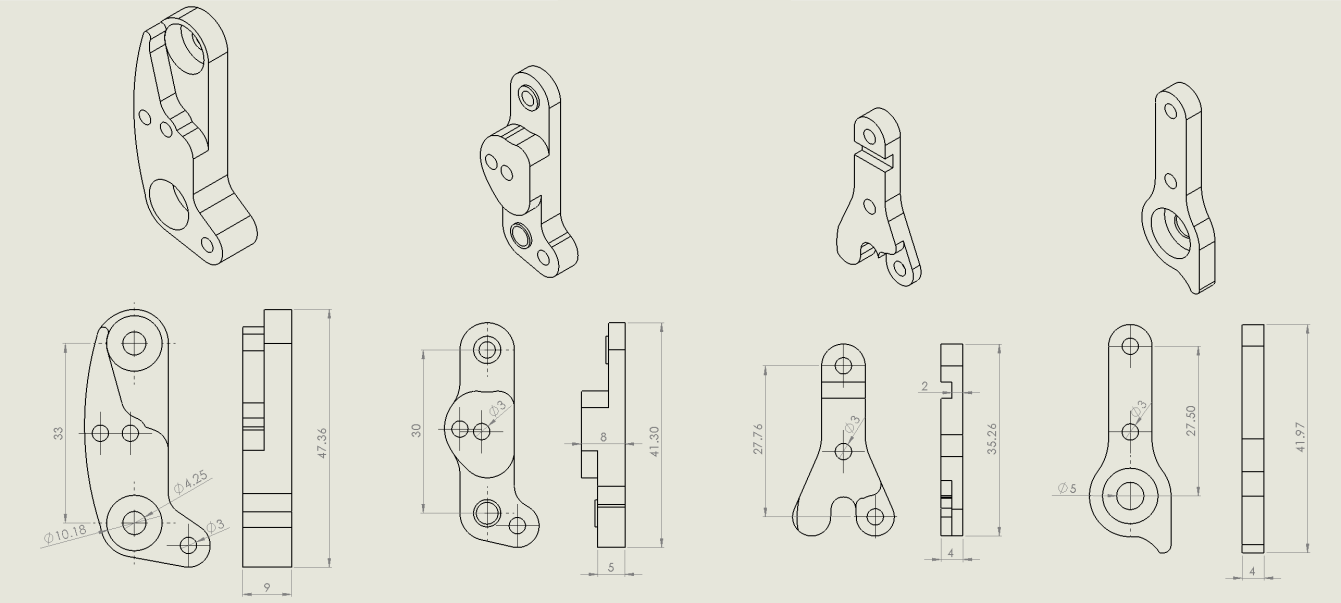
\includegraphics[width=0.9\textwidth]{Images/GripperDesign/dimensions.PNG}
    %\includegraphics[width=0.9\textwidth]{Images/placeholder.png}
    \caption{Drawing of 4 parts and their key dimensions, 2 of each part is needed for 1 finger}
    \label{fig:dimensions}
\end{figure}

\begin{figure}
    \centering
    \begin{subfigure}{.45\linewidth}
        \centering
        %\includegraphics[width=.4\textwidth]{Images/placeholder.png}       
        \includegraphics[width=0.9\textwidth]{Images/GripperDesign/8.JPG}
        \caption{Assembled Finger, View 1}
        \label{fig:AssFinger1}
    \end{subfigure}
    \begin{subfigure}{.45\linewidth}
        \centering
        \includegraphics[width=0.9\textwidth]{Images/GripperDesign/9.JPG}
        %\includegraphics[width=.4\textwidth]{Images/placeholder.png}
        \caption{Assembled Finger, View 2}
        \label{fig:AssFinger2}
    \end{subfigure}
    \begin{subfigure}{.45\linewidth}
        \centering
        %\includegraphics[width=.4\textwidth]{Images/placeholder.png}       
        \includegraphics[width=0.9\textwidth]{Images/GripperDesign/10.JPG}
        \caption{Assembled Finger, View 3}
        \label{fig:AssFinger3}
    \end{subfigure}
    \begin{subfigure}{.45\linewidth}
        \centering
        \includegraphics[width=0.9\textwidth]{Images/GripperDesign/11.JPG}          
        %\includegraphics[width=.4\textwidth]{Images/placeholder.png} 
        \caption{Exploded View}
        \label{fig:Exploded}
    \end{subfigure}
    \begin{subfigure}{.45\linewidth}
        \centering
        %\includegraphics[width=.4\textwidth]{Images/placeholder.png}       
        \includegraphics[width=0.9\textwidth]{Images/GripperDesign/12.JPG}
        \caption{Exploded view of 1 side of the finger}
        \label{fig:Explodedhalf}
    \end{subfigure}
    \begin{subfigure}{.45\linewidth}
        \centering
        \includegraphics[width=0.9\textwidth]{Images/GripperDesign/14.JPG}          
        %\includegraphics[width=.4\textwidth]{Images/placeholder.png} 
        \caption{4 distinct parts required}
        \label{label:}
    \end{subfigure}
    \label{fig:4Parts2}
    \caption{Parts and assemble of 1 finger}
    \label{figure:ViewsOf1Finger}
\end{figure}

\section{Actuation}
It was determined that for the purposes of the planned experiments which this gripper will be used for, that underactuation is sufficient to examine the relevant research questions. Using underactuation significantly simplifies the procedure and allows isolation of the variables under examination. As previously discussed underactuation is when the number of joints is greater than the number of actuators. When used in grasping, underactuaction gives the ability to self adapt to the object being grasped. This is achieved in this design by coupling each phalanx of the finger with an elastic element such that it will default to an open position. The design used mechanical limits to determine the relative orientation of each phalanx when open and therefore, determine the default finger position. A non-elastic element is then routed through the finger, as shown in figure \ref{figure:routing}, when actuated this will create a turning moment about each joint in turn. Starting with the bottom joint and ending with the top joint. This concept is more fully explored in Chapter \ref{LitReview} Section \ref{Actuation}\ref{UnderActuaction}

\begin{figure}
    \centering
    \begin{subfigure}{.45\linewidth}
        \centering
 %   \includegraphics[width=.4\textwidth]{Images/placeholder.png}       
    \includegraphics[width=0.7\textwidth]{Images/wirerouting/routing1.png}
        \caption{Step 1, Unactuated finger}
        \label{fig:routing1}
    \end{subfigure}
    \begin{subfigure}{.45\linewidth}
        \centering
        \includegraphics[width=0.7\textwidth]{Images/wirerouting/routing2.png}
%    \includegraphics[width=.4\textwidth]{Images/placeholder.png}
        \caption{Step 2, Bottom joint begins to curl}
        \label{fig:routing2}
    \end{subfigure}
    \begin{subfigure}{.45\linewidth}
        \centering
%    \includegraphics[width=.4\textwidth]{Images/placeholder.png}       
\includegraphics[width=0.7\textwidth]{Images/wirerouting/routing3.png}
        \caption{Step 3, Middle joint begins to curl}
        \label{label:routing3}
    \end{subfigure}
    \begin{subfigure}{.45\linewidth}
        \centering
        \includegraphics[width=0.7\textwidth]{Images/wirerouting/routing4.png}          
%    \includegraphics[width=.4\textwidth]{Images/placeholder.png} 
        \caption{Step 4, Tip joint begins to curl}
        \label{label:routing4}
    \end{subfigure}
    \caption{Shows routing of wire for underactuaction}
    \label{figure:routing}
\end{figure}
\chapter{Tactile Sensing} \label{Chapter:TactileSensing}
The tactile sensing fabricated and used in this research took inspiration from examples seen in the literature \cite{First3DHall,James}. It uses the hall effect to monitor the relative position of a hall effect sensor and a magnet. The magnets are embedded in a silicon rubber such that contact with the rubber will cause a deformation and a proportional change in magnet-sensor relative position. Magnets are embedded in silicon and placed over a hall effect sensor. An air gap between sensor and silicon is used to increase sensitivity \cite{HSSoft}.

\section{Material}
The material used was a "Polycraft T-15 Translucent Silicon Rubber" \cite{Silicon}. It is described by the manufacturer as a "two-component, high strength, flexible, moulding compound". It was found to be suitable for this application, since it is sufficiently robust so as to not deteriorate or change in performance after successive collisions during testing. It is sufficiently flexible, and of a suitable elasticity to act as a medium to suspend the magnet in such that a small force contacting the surface causes a detectable change in the relative sensor-magnet position. Finally, since it was a two-part compound it was easy to mould to a custom shape. The silicon remained liquid until and for approximately 20 mins after the two parts where mixed. This was sufficient time to fill and close the mold.

\section{Sensor}
The sensor used was an MLX90393 hall effect sensor \cite{MLX}. This particular sensor is highly suitable for this application and for this reason can also be seen in prior literature. The sensor is:
\begin{itemize}
    \item Small
    
    The MLX90393 is 3x3x1mm. This is particularly important since the tactile sensing is implemented onto the tip of a robotic gripper which is a size comparable to that of a human hand.
    \item Simple to implement
    
    The sensor itself has a lot of built in logic and can be interfaced with via the I2C communication protocol, making it simple to implement. Parameters such as the sample frequency, mode (burst, single measurement and wake-on-change), sensitivity, gain, etc. can be set and data collected using an appropriate microcontroller. Furthermore the I2C communication protocol allows two communication lines (SCL and SDA) to enable communication between many devices using 7-bit addressing. This reduces the number of wires which require routing through the gripper. This presents a significant advantage since the gripper has many joints which makes routing difficult and any gripper may have a large number of tactile sensors.
    \item High Sensitivity
    
    $0.294 \frac{\mu T}{LSB}$ is stated as the maximum sensitivity of the sensor (in the Z-axis). This is orders of magnitude too sensitive for this application and causes the 16 bit long reported data to overflow such that there are discontinuities in the sensor data over the range of reasonable contact forces. To overcome this both the on-chin gain and sensitivity are set lower so as the output is within a suitable range for the application. 
    \item Mutil-axis
    
    The sensor in question reports the magnetic field strength in all three axis (X, Y and Z). This is incredibly useful for tactile sensors implemented in a robotic gripper since it has the ability to report more than just forces perpendicular to the gripper but can also infer information about shear and non-normal forces. Theoretically this would give a gripper the ability to infer an objects weight, and surface characteristics as well as detect slippage and the angle of incidence of a collision to name a few examples. 
    
    \item High Frequency
    
    Since this project is exploring the grasping of moving objects the ability to sample sensors at a high frequency is of upmost importance. The sample frequency of this sensor is dependant on a number of variables and settings including the sensor mode, relevant axis, BURST\_DATA\_RATE, temperature, over-sample-rate of the ADC, etc. For this reason it is difficult to give a value for the max sample rate however it is in the order of tens of milliseconds per sample or 10-100Hz.
\end{itemize}

\section{Air-gap}
One feature of the design of the tactile sensors taken directly from prior literature is the use of an air gap between the sensor and magnet-silicon. An observation both from early stage testing of a prototype sensor and from the literature is that there is significant amount of cross talk between the axis when the silicon is deformed. Cross talk is when a force normal to the surface (in the z-axis) would cause significant changes in the magnetic field in the x and/or y axis. It was discovered that the mechanism causing this cross-talk was because the silicon was elastic but relatively incompressible. Therefore when a force would deform the compliant covering, the magnet would move both in the direction of the force but also in a direction perpendicular to the force because of the flow of the material. The solution to this was to add an air gap above the sensor. Since air is compressible, and also free to flow out of the cavity, the relative movement between magnet and sensor was more representative of the force causing the deformation. Furthermore the addition of an air gap significantly increased the sensitivity of the senors. The one downside of the air gap is the increased hysteresis, however this is not an issue in the application of grasping a moving object and so will not be a problem during the course of this research.

\begin{figure}
    \centering
    \begin{subfigure}{.45\linewidth}
        \centering
 %   \includegraphics[width=.4\textwidth]{Images/placeholder.png}       
    \includegraphics[width=0.7\textwidth]{Images/nogap.png}
        \caption{Without an air gap}
        \label{fig:nogap}
    \end{subfigure}
    \begin{subfigure}{.45\linewidth}
        \centering
        \includegraphics[width=0.7\textwidth]{Images/nogapforce.png}
%    \includegraphics[width=.4\textwidth]{Images/placeholder.png}
        \caption{Incomprehensibility causes unpredictable material flow }
        \label{fig:nogapforce}
    \end{subfigure}
    \begin{subfigure}{.45\linewidth}
        \centering
%    \includegraphics[width=.4\textwidth]{Images/placeholder.png}       
\includegraphics[width=0.7\textwidth]{Images/Airgap.png}
        \caption{Introduction of an air gap}
        \label{label:airgap}
    \end{subfigure}
    \begin{subfigure}{.45\linewidth}
        \centering
        \includegraphics[width=0.7\textwidth]{Images/airgapforce.png}          
%    \includegraphics[width=.4\textwidth]{Images/placeholder.png} 
        \caption{Displacement is in direction of the contactforce}
        \label{label:airgapforce}
    \end{subfigure}
    \label{figure:airgap}
    \caption{Shows the reason for cross-talk and the advantage of an air gap above the sensor}
\end{figure}

\section{Fabribation}
The sensor required two main fabrication methods, the printing of the PCB and the molding of the silicon rubber. The PCB, seen in Figure \ref{fig:PCB}, is a custom PCB which enables the I2C communication protocol and minimises all other wires. The manufacturing of this part was outsourced. 

The silicon was molded to a custom shape. To achieve this, molds where created from PLA using additive manufacturing, shown in Figures \ref{figure:moldCAD} \& \ref{figure:Molding}. The mold was made in two parts, the primary mold and a lid. The lid could be bolted into place and included the geometry to create an air gap and auto-alignment with the primary mold. The lid also had risers to allow excess silicon to flow out of the mold, ensuring that there were no unintentional air bubbles left in the silicon during the curing process. In order to hold the magnet in position during the curing process a small (1mm) drill bit was used to bore a hole in the bottom of the mold. The magnet could then to attached to the top of the drill bit and the drill bit friction fitted into place.

\begin{figure}
    \centering
    \includegraphics[width=0.7\textwidth]{Images/PCB.png}
    \caption{MLX90393 PCB}
    \label{fig:PCB}
\end{figure}

\begin{figure}
    \centering
    \begin{subfigure}{.3\linewidth}
        \centering
 %   \includegraphics[width=.4\textwidth]{Images/placeholder.png}       
    \includegraphics[width=0.7\textwidth]{Images/mold/exploded.png}
        \caption{Exploded View}
        \label{fig:exploded}
    \end{subfigure}
    \begin{subfigure}{.3\linewidth}
        \centering
%    \includegraphics[width=.4\textwidth]{Images/placeholder.png}       
\includegraphics[width=0.7\textwidth]{Images/mold/magnetoff.png}
        \caption{Drillbit in place}
        \label{label:Drillbitinplace}
    \end{subfigure}
    \begin{subfigure}{.3\linewidth}
        \centering
        \includegraphics[width=0.7\textwidth]{Images/mold/siliconout.png}          
%    \includegraphics[width=.4\textwidth]{Images/placeholder.png} 
        \caption{Magnet in place}
        \label{label:magnetinplace}
    \end{subfigure}
    \begin{subfigure}{.3\linewidth}
        \centering
        \includegraphics[width=0.7\textwidth]{Images/mold/lidoff.png}       
  %  \includegraphics[width=.4\textwidth]{Images/placeholder.png}
        \caption{Lid off}
        \label{fig:LidOff}
    \end{subfigure}
        \begin{subfigure}{.3\linewidth}
        \centering
        \includegraphics[width=0.7\textwidth]{Images/mold/unbolted.png}
%    \includegraphics[width=.4\textwidth]{Images/placeholder.png}
        \caption{Bolted, to compress the mold}
        \label{fig:unbolted}
    \end{subfigure}
    \begin{subfigure}{.3\linewidth}
        \centering
        \includegraphics[width=0.7\textwidth]{Images/mold/bolted.png}    
  %  \includegraphics[width=.4\textwidth]{Images/placeholder.png}
        \caption{Setting}
        \label{fig:Bolted}
    \end{subfigure}
    \caption{Computer Rendering of the silicon mold}
    \label{figure:moldCAD}
\end{figure}

\begin{figure}
    \centering
    \begin{subfigure}{.45\linewidth}
        \centering
 %   \includegraphics[width=.4\textwidth]{Images/placeholder.png}       
    \includegraphics[width=0.9\textwidth]{Images/mold/mold.png}
        \caption{3D printed silicon mold, 1}
        \label{fig:mold}
    \end{subfigure}
    \begin{subfigure}{.45\linewidth}
        \centering
        \includegraphics[width=0.9\textwidth]{Images/mold/moldinverted.png}
%    \includegraphics[width=.4\textwidth]{Images/placeholder.png}
        \caption{Mold, 2}
        \label{fig:MoldInverted}
    \end{subfigure}
    \begin{subfigure}{.45\linewidth}
        \centering
%    \includegraphics[width=.4\textwidth]{Images/placeholder.png}       
    \includegraphics[width=0.9\textwidth]{Images/mold/moldstanding.png}
        \caption{Mold, 3}
        \label{label:MoldStanding}
    \end{subfigure}
    \begin{subfigure}{.45\linewidth}
        \centering
        \includegraphics[width=0.9\textwidth]{Images/mold/drillinserted.png}          
%    \includegraphics[width=.4\textwidth]{Images/placeholder.png} 
        \caption{Drillbit in place}
        \label{label:drillInserted}
    \end{subfigure}
    \begin{subfigure}{.45\linewidth}
        \centering
        \includegraphics[width=0.9\textwidth]{Images/mold/withmagnet.png}       
  %  \includegraphics[width=.4\textwidth]{Images/placeholder.png}
        \caption{Magnet in place}
        \label{fig:withmagnet}
    \end{subfigure}
    \begin{subfigure}{.45\linewidth}
        \centering
        \includegraphics[width=0.9\textwidth]{Images/mold/closed.png}    
  %  \includegraphics[width=.4\textwidth]{Images/placeholder.png}
        \caption{Mold closed}
        \label{fig:closed}
    \end{subfigure}    
    \begin{subfigure}{.45\linewidth}
        \centering
        \includegraphics[width=0.9\textwidth]{Images/mold/withsilicon.png}       
  %  \includegraphics[width=.4\textwidth]{Images/placeholder.png}
        \caption{Resulting silicon}
        \label{fig:withSilicon}
    \end{subfigure}
    \begin{subfigure}{.45\linewidth}
        \centering
        \includegraphics[width=0.9\textwidth]{Images/mold/complete.png}    
  %  \includegraphics[width=.4\textwidth]{Images/placeholder.png}
        \caption{Complete, 1}
        \label{fig:complete}
    \end{subfigure}
    \begin{subfigure}{.45\linewidth}
        \centering
        \includegraphics[width=0.9\textwidth]{Images/mold/complete2.png}    
  %  \includegraphics[width=.4\textwidth]{Images/placeholder.png}
        \caption{Complete, 2}
        \label{fig:complete2}
    \end{subfigure}
    \caption{Images of the mold and molding process}
    \label{figure:Molding}
\end{figure}



\chapter{Tactile Reactive Control Strategy}\label{IROS2019}

This chapter outlines an experiment which tests and compares the performance of two approaches to grasping a moving object. This experiment specifically evaluates the tolerance for temporal and spacial errors for two different grasping strategies. The first approach (typical in the prior art) is a vision-only approach. Image sensors localise and track a target object as it moves, and open-loop control is used to close the gripper when the object is within a defined range. This approach acts as the control group to which the second approach is compared.

The second approach evaluated in this experiment explores if a performance improvement can be made by supplementing the vision system with tactile feedback from the gripper. The grasp reacts to feedback from tactile sensors located in the gripper (i.e. the motion of the gripper closing is dependant on how the object makes contact with it). If such a strategy was successful in increasing the tolerance for error, both temporal and spacial, in the estimate of an appropriate interception point along the target objects trajectory the computational overhead associated with grasping moving objects would be reduced. Since estimations can be less accurate and still result in a successful grasp. Furthermore, the need to place sensors in the environment to accurately track the target object's trajectory is removed and the problem can be tackled with on-board sensors. This allows such a solution to be deployed on a general purpose, mobile, service robot which cannot rely on an existing infrastructure of sensors and does not have vast quantities of computing power. 

\section{Reactive Strategy}\label{subsec:strategy}

The reactive tactile grasping is a novel approach, proposed in this research, and as such, needs to be tested and compared to the traditional approach prior to any further optimisation of the contribution of tactile feedback. Thus, such optimisations are outside the scope of this experiment and chapter but are addressed later in this document, as an area for future research. The grasping strategy used in this research was based on three basic rules:

\begin{enumerate}
    \item The grasp is triggered when the object first makes contact with the gripper (figures \ref{subfigure:Stage1} \& \ref{subfigure:Stage2}). This contrasts to the vision-only system which would close at the estimated interception time.
    \item The gripper attempts to reduce the spacial error by adjusting its position in the x-axis. Tactile sensors detect the point of contact and trigger the gripper to move along the x-axis accordingly . This is represented by arrow 1 in figure \ref{subfigure:Stage3}
    \item The finger which comes into contact with the object first delays its closing motion while the other finger begins to close, resulting in the grasp being slightly asymmetric as seen in Fig. \ref{subfigure:Stage4}. This offers an advantage over the vision-only system lacks the information about the contact point(s), preventing the grasping motion from being adapted to the object position. This is represented by arrow 2 in figure \ref{subfigure:Stage3}
\end{enumerate}

\begin{figure}[ht]
    \centering
    \begin{subfigure}{.45\linewidth}
        \centering
        \includegraphics[width=0.9\textwidth]{Images/stage1.png}
%  \includegraphics[width=.4\textwidth]{Images/placeholder.png}
        \caption{Stage 1}
        \label{subfigure:Stage1}
    \end{subfigure}
    \begin{subfigure}{.45\linewidth}
        \centering
        \includegraphics[width=0.9\textwidth]{Images/stage2.png}
%    \includegraphics[width=.4\textwidth]{Images/placeholder.png}
       \caption{Stage 2}
        \label{subfigure:Stage2}
    \end{subfigure}
    \begin{subfigure}{.45\linewidth}
        \centering
        \includegraphics[width=0.9\textwidth]{Images/stage3.png}
%    \includegraphics[width=.4\textwidth]{Images/placeholder.png}
        \caption{Stage3}
        \label{subfigure:Stage3}
    \end{subfigure}
    \begin{subfigure}{.45\linewidth}
        \centering
%    \includegraphics[width=.4\textwidth]{Images/placeholder.png}
    \includegraphics[width=0.9\textwidth]{Images/stage4.png}
        \caption{Stage 4}
        \label{subfigure:Stage4}
    \end{subfigure}
    \caption{Illustration of the simple tactile enabled, reactive grasping strategy: (a) Stage 1: Ball approaches gripper with a negative spacial offset in x,(b) Stage 2: Ball makes contact with gripper, a tactile sensor in the left finger triggers the grasp,(c) Stage 3: Gripper attempts to grasp the ball, its strategy is informed by tactile sensing,(d) Stage 4: Grasp is successful}
\label{fig:Tactile Stragety}
\end{figure}

\subsection{Experimental Setup}

The experiment involved the use of a two finger (each with 3 degrees of freedom) pincer gripper, outlined in Chapter \ref{Chapter:GripperDesign}, which was tasked with grasping a moving billiards ball. The grasper is actuated using servo motors controlled by an ESP32. Similarly the grasping strategy, outlined above, is implemented using the same ESP32 micro controller \cite{gitIROS}. The grasping unit was actuated in the x-direction (Fig. \ref{fig:Tactile Stragety}) along a linear rail using a servo motor. Each finger contained three tactile sensors, one on each flange, these tactile sensors are outlined in Chapter \ref{Chapter:TactileSensing}.

\begin{figure}[ht]
    \centering
    \begin{subfigure}{.8\linewidth}
        \centering
        \includegraphics[width=\textwidth]{Images/Dimensions.png}
%        \includegraphics[width=.4\textwidth]{Images/placeholder.png}
        \caption{Drawing of pincer gripper with dimensions}
        \label{subfig:1a}
    \end{subfigure}
    \begin{subfigure}{.8\linewidth}
        \centering
    \includegraphics[width=\textwidth]{Images/LabeledPhoto.png}
%    \includegraphics[width=.4\textwidth]{Images/placeholder.png}
       \caption{Photograph of pincer gripper used}
        \label{subfig:1b}
    \end{subfigure}
 \caption{Under-actuated, two finger, pincer gripper with distributed tactile sensing, a soft compliant covering, and joint position feedback.}
\label{fig:Gripper}
\end{figure}

A spherically shaped object was used as the moving grasp object since it presents the same grasping problem regardless of orientation. The target object, a billiards ball, was chosen because of its properties, namely high stiffness, spherical shape, size, mass and confidence in it manufacturing quality.

The object was set in motion by rolling down an inclined plane, similar to the method outlined in \cite{DynamicObjectManipulation}. In this setup, a long bar of aluminium with a U profile was used to control the object's trajectory toward the gripper (in the negative z-direction according to figure \ref{subfigure:RigDiagram}). The ball was forced to maintain this trajectory until just before coming within the range of the gripper where it was transitioned onto a horizontal planar surface. A photo and illustration of the control rig is given in figure \ref{fig:FullRig}. 

To ensure repeatability, the release of the ball was automated using servo motors. The speed of the ball was measured by monitoring the time the ball took to break two light gates, close to the gripper, placed at a known distance apart. The signals from the light gates were recorded by an independent system which used a logic analyser sampling at 2M samples/sec. Three different speeds were tested by releasing the ball from different heights on the inclined plane. The repeatability of this approach was validated prior to the experiment in a set of controlled tests and the readability monitored during testing by comparing measured speeds, this data is presented in table \ref{tab:repeatability}).

As outlined in chapter \ref{Chapter:GripperDesign}, the simplification of the gripper to an under-actuated, two-fingered, pincer gripper and the grasping problem to a two dimensional case enabled the elimination of many variables which might have effected the repeatability of the experiment without relevance to the research question. This enabled a controlled experiment to be conducted where the effect of the embedded tactile sensing in the gripper can be isolated. Although simplified, this system is analogous to more complex manipulators used in other setups. 

\begin{figure}[ht]
    \centering
    \begin{subfigure}{.8\linewidth}
        \centering
        \includegraphics[width=\textwidth]{Images/FinalRig.png}
%        \includegraphics[width=.4\textwidth]{Images/placeholder.png}
        \caption{}
        \label{subfigure:RigDiagram}
    \end{subfigure}
    \begin{subfigure}{.8\linewidth}
        \centering
    \includegraphics[width=\textwidth]{Images/RIG.png}
%    \includegraphics[width=.4\textwidth]{Images/placeholder.png}
        \caption{}
        \label{subfigure:RigPhoto}
    \end{subfigure}
    \caption{Experimental Rig, a) diagram and b) overhead photo}
\label{fig:FullRig}
\end{figure}

\subsection{Experiment Design} % perhaps procedure
This research compares two approaches to grasping a moving object. The first was an analog of the vision-only approach where the light gates are used to inform grasp timing, but the grasp itself is achieved in an open-loop fashion. The second system used tactile sensing, implemented by following the rules outlined in section \ref{subsec:strategy}.

For each approach, the gripper's ability to successfully grasp the moving object was evaluated (dependent variable) for  different speeds (three levels), different offset distances (five levels) and different grasping strategies (four levels). Ten tests were conducted for each condition. 

The basic format of each test was the same. The ball would be placed on the ramp and held in place by one of the release servos. The servo would release the ball, allowing it to accelerate down the ramp. The ball was then transitioned to the flat plane where the gripper would attempt to grasp it. After the attempt, the platform on which the ball was rolling was lowered to remove any force, external to the gripper, from supporting the ball. The grasp was deemed a success if the gripper was able to support the full weight of the ball and a failure otherwise. 

\begin{table}[ht]
\centering
\begin{tabular}{r|c|c|c}
\textbf{(m/s)}           & \textbf{Speed 1}       & \textbf{Speed 2}       & \textbf{Speed 3}       \\
\hline
Mean                   & 0.82363 & 0.96363 & 1.08727   \\
Standard Deviation     & 0.01305 & 0.01252 & 0.02127   \\
Standard Error         & 0.00092 & 0.00089 & 0.00150   \\
%Confidence Level (95\%)       & 0.00182 & 0.00175 & 0.00297   \\
Number of Measurements & 200     & 200     & 200 
\end{tabular}
\caption{Speed data for 600 tests at 3 different speeds}
\label{tab:repeatability}
\end{table}

\section{Results}

Tests were conducted for three variations of the vision-only condition; each variation represented a different timing trigger from the point at which the ball passed the light gate. These timings (0ms, 5ms, 10ms) were determined empirically to represent fast, medium, and slower open-loop response conditions. In contrast, the test for the reactive grasping condition does not account for the three timings, since sensor stimulus triggers an near-instant response. The results across all of the test conditions are presented in figure \ref{fig:Results}, displaying the success rate under each set of conditions.

Analysis was performed to evaluate the influence of grasping strategy and spacial offset on grasp reliability across the range of object velocities. The success rates of the open-loop (OL) grasping strategy, for the three timings, and the reactive grasping strategy is shown in figure \ref{fig:meangraph}.

\begin{figure}[ht]
    \centering
    \includegraphics[width=0.475\textwidth]{Images/resultsgraph.png}
    \caption{Mean number of successful grasps per grasping strategy across all tests.}
    \label{fig:meangraph}
\end{figure}%

\begin{figure}[ht]
    \centering
    \includegraphics[width=0.9\textwidth]{Images/CrosslandResults.png}
    \caption{Representation of the grasping success rate based on stragety}
    \label{fig:CrosslandGraph}
\end{figure}%

\begin{figure}[ht]
    \centering
    \begin{subfigure}{.3\linewidth}
        \centering
        \includegraphics[width=\textwidth]{Images/VisionResults0.png}
%        \includegraphics[width=.4\textwidth]{Images/placeholder.png}
        \caption{Time Offset 0ms}
        \label{subfigure:TimeOffset0ms}
    \end{subfigure}
    \begin{subfigure}{.3\linewidth}
        \centering
    \includegraphics[width=\textwidth]{Images/VisionResults5.png}
%    \includegraphics[width=.4\textwidth]{Images/placeholder.png}
        \caption{Time Offset 5ms}
        \label{subfigure:TimeOffset5ms}
    \end{subfigure}
    \begin{subfigure}{.3\linewidth}
        \centering
        \includegraphics[width=\textwidth]{Images/VisionResults10.png}
%        \includegraphics[width=.4\textwidth]{Images/placeholder.png}
        \caption{Time Offset 10ms}
        \label{subfigure:TimeOffset10ms}
    \end{subfigure}
    \hfill
    \begin{subfigure}{.3\linewidth}
        \centering
        \includegraphics[width=\textwidth]{Images/Tactile.png}
%        \includegraphics[width=.4\textwidth]{Images/placeholder.png}
        \caption{Tactile Sensing System}
        \label{subfigure:TactileSensingSystem}
    \end{subfigure}
    \caption{Successful grasp rates, observed over 10 tests under each set of conditions}
\label{fig:Results}
\end{figure}

The grasp reliability data was analyzed with a two-way factorial ANOVA. Significant (p $\leq$ 0.01) effects were found for the main effect of grasp strategy, F(3, 40) = 5.8049, p \textless 0.01 and grasp offset F(4, 40) = 25.8232, p \textless  0.01. A significant effect was also found for interaction between grasp strategy and positional offset, F(12, 40) = 7.0752, p \textless  0.01. A post hoc Tukey test, performed on the interaction effect, revealed significant differences at the highest offset value (i.e. spacial offset = 60mm) indicating that that the reactive grasping strategy outperformed each of the open loop strategies, p\textless0.01.

\section{Discussion}

% Speed has only a moderate effect on the visions systems ability to grasp while its effects are more pronounced for the tactile system due to inherient time error 
The results suggest that the vision-only system performs best at low spacial and temporal offsets. In this context, speed has a moderate effect on the grippers ability. In contrast, the effect of speed is greater for the reactive system. The grasping success rate is consistently poorer at higher speeds for this system. This highlights the importance of reaction time to this approach. The tactile strategy requires stimulus from contact between object and gripper to trigger the grasp whereas the vision-only system relies on an estimate interception time. However, the optimum grasp time is before contact between object and gripper. As a result, the tactile system has a small, inherent temporal offset from optimal. Therefore, the reduction in the time to react caused by a faster moving object, has a larger impact on the rate of successful grasping. 

%Temporal error can not grow
The first advantage offered by the tactile approach is observed when compared  to the visual system with a 10ms temporal offset. The tactile system significantly outperforms the visual system under these conditions, despite the inherent temporal error in the tactile approach. Since the tactile approach is reacting to real-world interaction between object and gripper the temporal error remains relatively small as opposed to an estimation from a vision system. 

% Tactile system outperforms visual system for the largest spacial offset (60mm)
The second advantage of the tactile, reactive control approach is observed when examining the effects of spacial offset. Grasping success rate for the vision-only approach consistently worsened as x-offset increased. The average success rate for all speeds and temporal offsets dropped to 3.3\% at a spacial offset of 60mm. The proposed tactile grasping strategy performs better with a 93.3\% success rate at a 60mm offset. 

% Sparse tactile sensing
A further finding of this research is the importance of the density of the tactile sensing, when using it in this context. The fingers used in this testing had just six tactile sensors, one placed in each flange of each of the fingers. This caused some inconsistencies in performance, for example the tactile approach preformed worse on average at no offset, 15mm and 45mm offsets than at 30mm and 60mm. It would seem appropriate that a lower offset from optimum would yield a higher success rate. However due to the sparsity of tactile sensors there were particular offsets which would allow the gripper to detect the presence of the ball and react faster than others. This would result in a higher grasping success rate. Higher-density sensor system have been demonstrated in prior literature \cite{uSkinFingertip}\cite{Allegro} and might yeild still better results. 

% Inhomogeneous
A factor which further contributes to this effect is the irregular shape and inhomogeneous surface of the fingers. The result of which is a complex interaction between object and gripper which is dependant on offset in a non linear way. Since the tactile approach relies on such an interaction to trigger the grasp, the nature of that interaction and subsequent rebound play a role in achieving a successful grasp. 

A specific example the effect of sparse tactile sensing and inhomogeneity can be seen in the observed success rate (50\%) of the tactile system at high speed and no spacial offset. These set of conditions resulted in contact between ball and gripper between the two fingers. In this position there is neither tactile sensing nor silicon to absorb any kinetic energy. The resulting rebound carried the ball out of range of the gripper before a successful grasp 50\% of the time. This suggests that these poor results are likely attributable to limitations of the experimental hardware, not the approach.

\section{Conclusions}
This chapter outlines research which proposed a novel grasping strategy for dynamic objects informed by tactile sensing. It argued that reacting to tactile feedback enables the gripper to alter its position and grasping motion, so as to achieve higher successful grasping rates. Results presented here confirm that tactile sensing can contribute to a better grasping strategy. The gripper successfully grasped the object at greater spacial offsets when employing the tactile feedback to inform its motion. Despite an inherent temporal error in the tactile grasping strategy, the response time was sufficient to react to spacial errors and grasp the object,
%maybe compare to vision here 
due to the reactive nature of the tactile approach. The findings from this research motivate further research, which are outlined in the next chapter

\chapter{Future Work and Conclusion}

The remaining research which will be conducted during the course of this project can be described as four work packages, each with an associate research question and submission for publication. Each explores an avenue to further examine how sensing can be used to enable the gripper motion while grasping moving objects. Appendix \ref{Gantt1} - \ref{GanttBreakdownmisc} shows a more detailed outline of how the remaining time in the project will be used to complete these work packages. These work packages are:
\begin{itemize}
    \item Neural network trained using reinforcement learning to map tactile sensor stimilius to gripper motion while grasping moving objects.
    \item The role vision sensor placement plays in grasping moving objects
    \item A proposal for a holistic visuotactile strategy for grasping moving objects
    \item Remote tactile sensing as a strategy to inform grasping motion
\end{itemize}

\section{Neural Networks and Reinforcement Learning} \label{RL}

%% Justify research, connect it to existing research

This work would build on the previous submission to IROS2019 where it was concluded that tactile sensing could positively contribute to the motion of a gripper as it grasped a moving object. In that research, a simple rule based strategy was used to take advantage of tactile sensors. It was identified that this was not an optimisation of the potential contribution of tactile sensors and merely a proof of concept. To further this, research would be conducted with the aim of optimising the contribution of tactile sensors using a reinforcement learning approach.

% What is the research
Tactile sensing has already been shown to positively contribute to the motion of the gripper while grasping a moving object. However, there is no obvious way in which to couple actuation to sensor stimulus so as to optimise the contribution of tactile sensing. A deep neural network can be trained to couple sensor data to gripper movement, using reinforcement learning. The performance of the system controlled by a neural network can then be compared to systems with the same sensing capabilities but with a simple rule based strategy, i.e. the system outlined in the submission to IROS2019, and to a system which relies solely on an estimated interception position and time. This research hypothesises that a neural network trained using reinforcement learning can optimise the contribution of tactile sensing when grasping a moving object, outperforming existing systems with similar levels of sensing.

% How am I going to achieve this.
To enable training, through reinforcement learning, grasping attempts will be conducted, both in simulation and in the real world. Real world training will use an adapted version of the experimental rig outlined previously, while gazebo will be used for simulation. Training will start in simulation, since it is easier to achieve a high number of training cycles. This will allow quick iteration toward a suitable network architecture, hyper-parameters, etc. Training will then move to real world training, this will prevent over-fitting of the network to the idealised system in simulation. It is unclear as of yet if transfer learning can be used to take the trained network from simulation and retrain it in the real world or if it would be better to train from the beginning on the real world system. Further research into industry best practice, prior research and transfer learning theory is required before making that decision. The computational hardware used will be either an ESP32 or a Raspberry Pi. Both are suitable platforms with an ESP32 being the more appropriate option for lightweight, low-power, computation at-the-edge robotics and Raspberry Pi being more computationally powerful and therefore potentially a simpler way to address the research question. The complexity of the required neural network architecture and the number of required training epochs will determine which platform is used.

% Methodology
When fully implemented a methodology very similar to that outlined in chapter \ref{IROS2019} will be employed. Data about the grasping success rate will be collected for each system under various conditions, i.e. combinations of spacial offsets and speeds. 

\section{Vision Sensor Placement}\label{Vision}

%% Justify research, connect it to existing research
As discussed in previous chapters, vision is a fundamental part of any general purpose gripping solution. The problems associated with relying solely on vision has also been discussed. Vision is typically computationally expensive and therefore latency often renders it unsuitable for time critical applications. It is also vulnerable to occlusion and changes in lighting conditions. Until this point assumptions were made that a vision based system would place the actuator within grasping range of the target object, and the focus of research has been to increase the size of that grasping range, both temporally and spatially, and to reduce the reliance on a vision system. Any contributions which vision might make to the grasping motion itself has been largely ignored. This will now be examined in more detail.

% What is the research
This research explores the contribution image sensors have toward the grasping motion when the target object is dynamic, and specifically strives to understand the role camera placement plays in this. To investigate, a moving object will be grasped both in simulation and in real world experiments. Existing literature will be used to identify common problems with camera placement on-robot, i.e. occlusion, latency, lighting conditions, etc. Simulation will be used to explore how these issues can be tackled using camera placement, most likely in wrist, fingers and other arm. A real world system, with a short-list of camera placements (identified from simulation), will then be created and tested. Performance of systems using difference combinations of camera placements can then be compared.

% How am I going to achieve this.
Real world testing will be conducted on an adapted version of the existing testing apparatus, described in Chapter \ref{IROS2019} while testing in simulation will use Gazebo and the model developed for the previous reinforcement learning research discussed in section \ref{RL}. The cameras used will be the PiCam for the Raspberry Pi or the ESP32Cam. For similar reasons to those outlined in section \ref{RL} the decision of which platform has not been made yet. The ESP32 being more suitable for robotics, low power, lightweight, at the edge, applications but the Raspberry Pi being more computationally powerful. It will therefore depend on which algorithms and methods prove effective during simulated testing and how suitable each platform is to each approach. Implementation will rely heavily on available algorithms, source code, etc such as OpenCV and the ESP-IDF, which will also play a role in choosing the appropriate platform.

% Methodology
Echoing the experiments previously conducted, this exploration of the role sensor placement plays in grasping moving objects will culminate in real world testing. Image sensors will inform a grasping motion on a gripper and the performance of the gripper in terms of grasping success rate will be used to address the research question.

\section{ViseoTactile Grasping Strategy}

%% Justify research, connect it to existing research
Until this point, research has investigated independently how both tactile and vision sensing can be used to inform the motion of robotic fingers whilst grasping a dynamic object. Having investigated and optimised the contribution of both sensing mechanisms, this research aims to present a combined visuotactile system which can outperform the current state of the art as described in prior literature. 

% What is the research
The system should be robust to object shape, size and stiffness as well as velocity, angle of incidence, and spin. The tactile enabled reactive control strategy, powered by a neural network and reinforcement learning, outlined in section \ref{RL} , will be coupled with the learning's from the vision sensor placement research, outlined in section \ref{Vision}, to create a robotic gripper which employs a sensor-informed grasping motion. The grasp success rate for each combination of variables will be reported.

% How am I going to achieve this.
This work package relies heavily upon outcomes from the previous two. The realisation of a neural network to optimise the contribution of tactile sensing and a system with optimally implemented, in-hand cameras, is essential to realise the complete visuotactile system. Furthermore, a more complex testing apparatus will be required to allow the systems ability to handle objects of different shapes, spins, etc, to be tested. The gripper itself however will remain an adapted version of the existing gripper. Being a two-fingered pincer gripper, its simplicity allows for a robust, repeatable testing procedure and is sufficient to address the research question since the same principles could be extrapolated for more complex grippers.


\section{Remote Tactile Sensing}

%% Justify research, connect it to existing research
There has been little exploration of the potential contributions of alternative sensing mechanisms to the problem of grasping moving objects. Existing approaches rely heavily on image sensing. A reactive grasping stragety, enable by tactile sensing, has previously been proposed, see chapter \ref{IROS2019}. However a fundamental limitation of tactile sensing for this application was identified during that research. Traditional tactile sensing requires physical contact between object and gripper before a reaction to the sensor stimulus is possible. Since the optimum time to initiate a grasp is before contact between gripper and target object, a grasp reactive to tactile sensing alone has an inherent temporal offset from optimum which cannot be overcome. This research aims to address this barrier.

% What is the research
An investigate is conducted into alternative sensors which can provide accurate location information about the object, similar to that provided by tactile sensors, before contact with the gripper. Such a sensor would enable a grasping motion reactive in real-time to sensor data about object position. During this research the sensor, or several sensors using different mechanisms, would be created and implemented onto the existing gripper. Testing would be conducted on these systems to determine the effectiveness of this strategy, and to compare the different approaches to creating such a sensor.

% How am I going to achieve this.
Inspiration for appropriate sensors would be largely taken from prior literature where there are already examples of such sensors and details of how they have previously been created \cite{FingertipEmitterReceiverMovingObject, FingertipEmitterReceiverMovingObjectII}. The gripper and testing apparatus used would be very similar to that described in chapter \ref{IROS2019} since the research question is fundamentally the same but with a different sensor. The grasping strategy may be the simple rule based one previously described, since this is sufficient to address the research question, but neural networks and reinforcement would also be an option depending on how much overhead and development time would be deemed to be involved in such an approach. 

\section{Conclusion}
This document has outlined in detail this research project. Describing progress and findings to date as well as specifically outlining future research questions and a plan to address them. Through examination of the literature, determining how sensing can be used to inform a better, more informed grasping motion was identified as an under-explored and valuable area of research to pursue. To-date in this project, experiments have been conducted to examine the contribution that tactile sensing plays in informing a grippers motion when grasping a moving object. It was found that real-time tactile sensor data can be used to react to errors/offsets from optimum in the interception position and time between gripper and object and improve the grasp success rate over a range of variables. Future work, outlined above, aims to optimise this contribution aswell as examine other types of sensing, such as image sensing and remote tactile sensing. Finally, this project aims to present a holistic, visuo-tactile grasping strategy and an associated gripper which is capable of grasping moving objects, despite large errors in the estimated interception point, where sensor contribution is optimised.
\chapter{Appendix}
\appendix
\newpage
\section{Gantt Chart, part 1}\label{Gantt1}
\begin{figure}[h!]
    \centering
    \includegraphics[width=0.93\textheight, angle=270]{Images/GanttChart/Gantt1.png}
%    \caption{Gantt Chart outlining future work, Part 1}
%    \label{Gantt1}
\end{figure}
\newpage
\section{Gantt Chart, part 2}\label{Gantt2}
\begin{figure}[h!]
    \centering
    \includegraphics[width=0.93\textheight, angle=270]{Images/GanttChart/Gantt2.png}
%    \caption{Appendix 2: Gantt Chart outlining future work, Part 2}
%    \label{Gantt2}
\end{figure}

\newpage

\section{Gantt Breakdown, Work Package 1}\label{GanttBreakdownWP1}
\begin{itemize}
    \item Literature Review
    
    Read the relevant literature to ensure understanding of the state of the art and check validity of the research question.
    \item Software Setup
    
    Software installation and configuration. Tensorflow, Keras, Gazebo, Blender.
    \item Basic RL example 
    
    Run simple sample program which uses RL, this will be the mountain car problem provided in tensorflow. This will refresh machine learning knowledge and get familiar with the tools and any updates since I last used them.
    \item Complete Simulated Environment 
    
    Complete simulation of the gripper in gazebo. Configure gazebo such that the program can be launch and (unattended) it will run the grasp test iteratively and feed the results into tensorflow for RL. This is essential to achieve the large number of training cycles which is required to make RL feasible.
    \item Choose a Network Architecture
    
    Use existing research and ask people I know in the area to help choose a suitable or a short list of suitable existing neural network architectures for this application.
    \item Run Training in Simulation
    
    Start running training using the simulation. Starting with simulation will allow quick iteration on network architecture, training parameters, etc.
    \item Overcome Hardware shortfalls
    
    Several shortcomings where identified in the experimental rig used for testing for submission in IROS2019. These should be addressed before the same experimental setup is reused.
    \item Neural Network on ESP32 vs RPi
    
    Decide, through experimentation if necessary and documentation if possible, wether to continue development on an ESP32 or a Raspberry Pi
    \item Hardware for real-world training 
    
    The existing gripper will be set up and configured so that it is being controlled by the network in training. This includes the network-rig integration and the sensor integration.
    \item Explore Transfer Learning
    
    Decide if transfer learning is a viable and/or effective option, using experimentation and literature
    \item Real-world training
    
    Taken the lessons learnt from training in simulation into account, training on the real world robotic system will begin. It will take much longer to achieve the same number of training cycles in the real world relative to simulation and therefore some of the complications should be ironed out first in simulation
    \item Write submission for JIRS
    
    JIRS has been identified as a suitable publication to submit to. It is particularly relevant for the research since it focuses on inteligent control, mobile robots, sensors, sensor-fusion and sensor based control.

\newpage

\section{Gantt Breakdown, Work Package 2}\label{GanttBreakdownWP2}
    \item Literature Review
    
    Read the relevant literature to ensure understanding of the state of the art and check validity of the research question.
    \item Implement cameras in simulation
    
    Adapt simulation used in previous work package and implement cameras in different locations. Tip of the finger, wrist, robot torso and robot head. Implement basic computer vision, ball tracking algorithms.
    \item Role of camera location in simulation
    
    Address the core research question through simulation. What is the effect of the location of the camera, accounting for occulusion, resolution, processing speed, latency, implementation concerns, etc.
    \item Implement real world cameras
    
    Integrate ESP32 cam on existing experimental rig.
    \item Real world testing
    
    Verify findings of simulation testing on the experimental rig.
    \item Write Submission for IEEE Mag
    
    IEEE Robotics and Automation Magazine has been identified as a suitable candidate for publication of this research. They have a high impact factor and “focus on working systems and encourage creative solutions to real-world problems and highlighting implementation details”

\newpage

\section{Gantt Breakdown, Work Package 3}\label{GanttBreakdownWP3}
    \item Literature Review
    
    Read the relevant literature to ensure understanding of the state of the art and check the validity of the research question.
    \item Setup necessary hardware
    
    Set up gripper and testing rig with the necessary sensors, etc.
    \item RL Training on new system
    
    Train the new robotic system using Reinforcement learning
    \item Experimental Testing
    
    Benchmark the neural network against a similar network without vision and without tactile. Benchmark against a system using a rule based grasping stragety.
    \item Write Submission for IJRR
    
    IJRR has been identified as a suitable publication for this research as it is currently envisioned. IJRR is the highest ranked robotics journal and this publication would be the culmination of all research in this project to date, combining tactile sensing, reactive grasping, vision sensing and reinforcement learning.
    
    \newpage
    
\section{Gantt Breakdown, Work Package 4}\label{GanttBreakdownWP4}
    \item Literature Review
    
    Read the literature to ensure understanding of the state of the art and check the validity of the research question.
    \item Sensor(s) Manufacture
    
    Develop the sensor(s) which will tested as part of this work package. Light, sonar and wifi are all sensors I would like to test but still need to research the feasibility of each of these.
    \item Sensor(s) characterisation
    
    It is important to properly test the sensor and determine its accuracy, robustness, precision, latency, etc.
    \item Reconfigure Testing Rig
    
    Integrate sensor on gripper and ready the testing rig for testing
    \item Experimental Testing
    
    Conduct real world testing to access the usfullness of a remote tactile sensor to informing the grasping motion for grasping moving objects
    \item Write submissions for ICRA
    
    Identified as a suitable conference with a submission deadline around the correct time of year (~September).

    \newpage

\section{Gantt Breakdown, Misc}\label{GanttBreakdownmisc}
    \item Absent
    
    Foreseeable trips, hoildays, etc.
    \item Thesis Writeup
    
    6 months set aside for writing my final thesis document.

\end{itemize}







%% This defines the bibliography file (main.bib) and the bibliography style.
%% If you want to create a bibliography file by hand, change the contents of
%% this file to a `thebibliography' environment.  For more information 
%% see section 4.3 of the LaTeX manual.
\begin{singlespace}
\bibliography{main}
\bibliographystyle{plain}
\end{singlespace}


\end{document}

